\documentclass[11pt,a4paper]{article}
\usepackage[margin=22mm,headheight=14pt]{geometry}
\usepackage{fontspec}
\usepackage[fontset=none]{ctex}
\setmainfont{texgyrepagella-regular.otf}[BoldFont=texgyrepagella-bold.otf,ItalicFont=texgyrepagella-italic.otf,BoldItalicFont=texgyrepagella-bolditalic.otf]
\setsansfont{texgyreheros-regular.otf}[BoldFont=texgyreheros-bold.otf]
\setmonofont{lmmono10-regular.otf}[Scale=.87,BoldFont=lmmonolt10-bold.otf,ItalicFont=lmmono10-italic.otf,BoldItalicFont=lmmonolt10-boldoblique.otf]
\setCJKmainfont{FandolSong-Regular.otf}[BoldFont=FandolSong-Bold.otf]
\setCJKsansfont{FandolHei-Regular.otf}
\setCJKmonofont{FandolFang-Regular.otf}
\usepackage{booktabs,tabularx,array,longtable,amsmath,graphicx,xcolor,pdfpages}
\usepackage{tikz}
\usetikzlibrary{positioning,arrows.meta,calc}
\usepackage{listings,enumitem,fancyhdr,titlesec}
\usepackage{xurl,tocloft}
\setlength{\cftbeforesecskip}{4pt}
\usepackage[unicode,hidelinks]{hyperref}
\definecolor{accent}{HTML}{1D4B60}
\definecolor{soft}{HTML}{F0F4F6}
\hypersetup{pdftitle={Ride-Hailing Platform Database Design},pdfauthor={}}
\titleformat{\section}{\Large\bfseries\color{accent}}{\thesection}{.65em}{}
\titleformat{\subsection}{\normalsize\bfseries}{\thesubsection}{.6em}{}
\titlespacing*{\section}{0pt}{0pt}{12pt}
\setlength{\parindent}{0pt}
\setlength{\parskip}{7pt}
\renewcommand{\arraystretch}{1.3}
\setlength{\tabcolsep}{4pt}
\newcolumntype{Y}{>{\raggedright\arraybackslash}X}
\setlist{nosep,leftmargin=1.5em}
\lstset{basicstyle=\ttfamily\small,breaklines=true,columns=fullflexible,keepspaces=true,showstringspaces=false,backgroundcolor=\color{soft},frame=single,rulecolor=\color{soft},xleftmargin=6pt,xrightmargin=6pt,aboveskip=8pt,belowskip=8pt}
\pagestyle{fancy}\fancyhf{}\fancyfoot[C]{\small\thepage}
\fancyhead[L]{\small\sffamily Ride Hailing Database Design}
\fancyhead[R]{\small\sffamily G6 · Design and validation}
\renewcommand{\headrulewidth}{.3pt}
\emergencystretch=2em
\raggedbottom
\setcounter{tocdepth}{1}\titlespacing*{\subsection}{0pt}{13pt}{7pt}\titlespacing*{\subsubsection}{0pt}{10pt}{5pt}
\begin{document}\begin{titlepage}\thispagestyle{empty}\centering\vspace*{2cm}
{\fontsize{26}{34}\selectfont\bfseries Ride-Hailing Platform\\[4pt]Database Design\par}\vspace{1.1cm}
{\Large Group G6\par}\vspace{1.2cm}
\par\begingroup\small\noindent
\begin{tabularx}{\linewidth}{p{2cm}p{4cm}p{4cm}}
\toprule
Member & Student ID & Name\\\midrule
1 & 226040384 & Lin Shuaiyu\\
2 & 226040421 & Cai Ruihe\\
3 & 226040351 & Li Songzi\\
4 & 226040373 & Wen Zhang\\
5 & 226040424 & Zhang Xiujie\\
6 & 122090871 & Jin Conghao\\
\bottomrule
\end{tabularx}
\par\endgroup
\end{titlepage}\pagenumbering{roman}
\renewcommand{\contentsname}{Contents}
\begingroup\small\setlength{\parskip}{0pt}\tableofcontents\endgroup\clearpage\pagenumbering{arabic}
\section{Introduction and Requirements Analysis}
\subsection{Business context and scope}
A ride-hailing platform must relate a booking to its passenger, assigned vehicle, responsible driver and final outcome. This project builds a relational database for that operational record. It retains the original design's user roles, vehicles, insurance, shifts, trips and feedback, while making their keys, state rules and implementation consistent.

The primary users are passengers who request rides, drivers who serve them, and platform operators who inspect service records. The database supports registration, vehicle and policy registration, shift logging, trip assignment, start, completion, cancellation, fare details and feedback. It also supports operational queries and a small analytical snapshot. A front-end application is outside the deliverable.

The scenario is deliberately bounded. Vehicle ownership is fixed during the observation period; a driver may own several vehicles, but each vehicle has exactly one driver. A trip serves one passenger account. Shared rides, pooled passengers, driver substitutions and ownership history are excluded. These assumptions keep the original project manageable and make the functional dependencies explicit.

Fare records describe charges associated with completed trips. They are not payment confirmations, platform revenue or driver settlement statements. Payment gateways, recharge, refunds, real-time GPS, route optimization and regulatory eligibility verification are future extensions. No claim about legal driver eligibility follows from this teaching model.

The implementation uses MySQL, matching the SQL lectures. It contains 11 operational tables, two views, four lifecycle procedures, three guard triggers and an application role. Four additional tables form an analytical snapshot. All sample records are synthetic. The analysis illustrates what can be computed; it is not evidence about an actual ride-hailing business.


\subsection{Requirements and functional structure}
Each requirement is connected to a persistent object and an observable check. The database is judged by whether it represents the stated rules and rejects inconsistent changes, rather than by the number of entities alone. The course project specification requires the full development process and discussion; it does not prescribe a minimum table count.

A newly registered user may have no operational role yet. Passenger and driver roles can overlap. This supports a driver booking a ride as a passenger without duplicating their contact information. A booking exists before a vehicle is assigned, which makes optional participation necessary.

Insurance and shift records are stored for inspection and analysis. This version does not automatically reject assignment outside a shift or after insurance expiry. It also does not prevent two different trips being assigned simultaneously to one driver. Those are explicitly separate scheduling and dispatch constraints, not silently claimed features.

\par\begingroup\small\noindent
\begin{tabularx}{\linewidth}{p{.8cm}p{5cm}Y}
\toprule
ID & Requirement & Objects and verification\\\midrule
R1 & Shared identity and overlapping roles & app\_\allowbreak{}user, passenger, driver; one overlapping account\\
R2 & Vehicle and insurance records & vehicle, insurance\_\allowbreak{}policy; immutable owner and date checks\\
R3 & Multiple shifts per day & driver\_\allowbreak{}shift; composite key and chronological checks\\
R4 & Request and assign a vehicle & trip; request default, driver/vehicle match\\
R5 & Mutually exclusive terminal outcomes & completed\_\allowbreak{}trip, cancelled\_\allowbreak{}trip; procedures and guards\\
R6 & Fare components and two-sided feedback & surcharge, review; exact decimals and score checks\\
R7 & Operational and analytical queries & views and warehouse; counts, sums and query outputs\\
R8 & Reproducible implementation & seed, SQL, tests and saved machine-readable results\\
\bottomrule
\end{tabularx}
\par\endgroup

The next two diagrams restore the functional decomposition of the original design. Passenger and driver services are separated on the front end; identity, assets, operations, finance and location are organized on the back end. These are requirement diagrams, not screenshots of an implemented application.

Solid boxes identify functions supported by the implemented database. Gray boxes preserve related services from the initial business description while marking them as external or future work. Registration records are stored, but login authentication is not implemented. Fare records and summaries are implemented, but payment execution and settlement are not. Driver identity is recorded, while formal eligibility review remains external.

This scope distinction prevents the diagrams from promising functionality absent from the schema. It also preserves the broader ride-hailing context without expanding the current database beyond its 11 core tables.

\clearpage
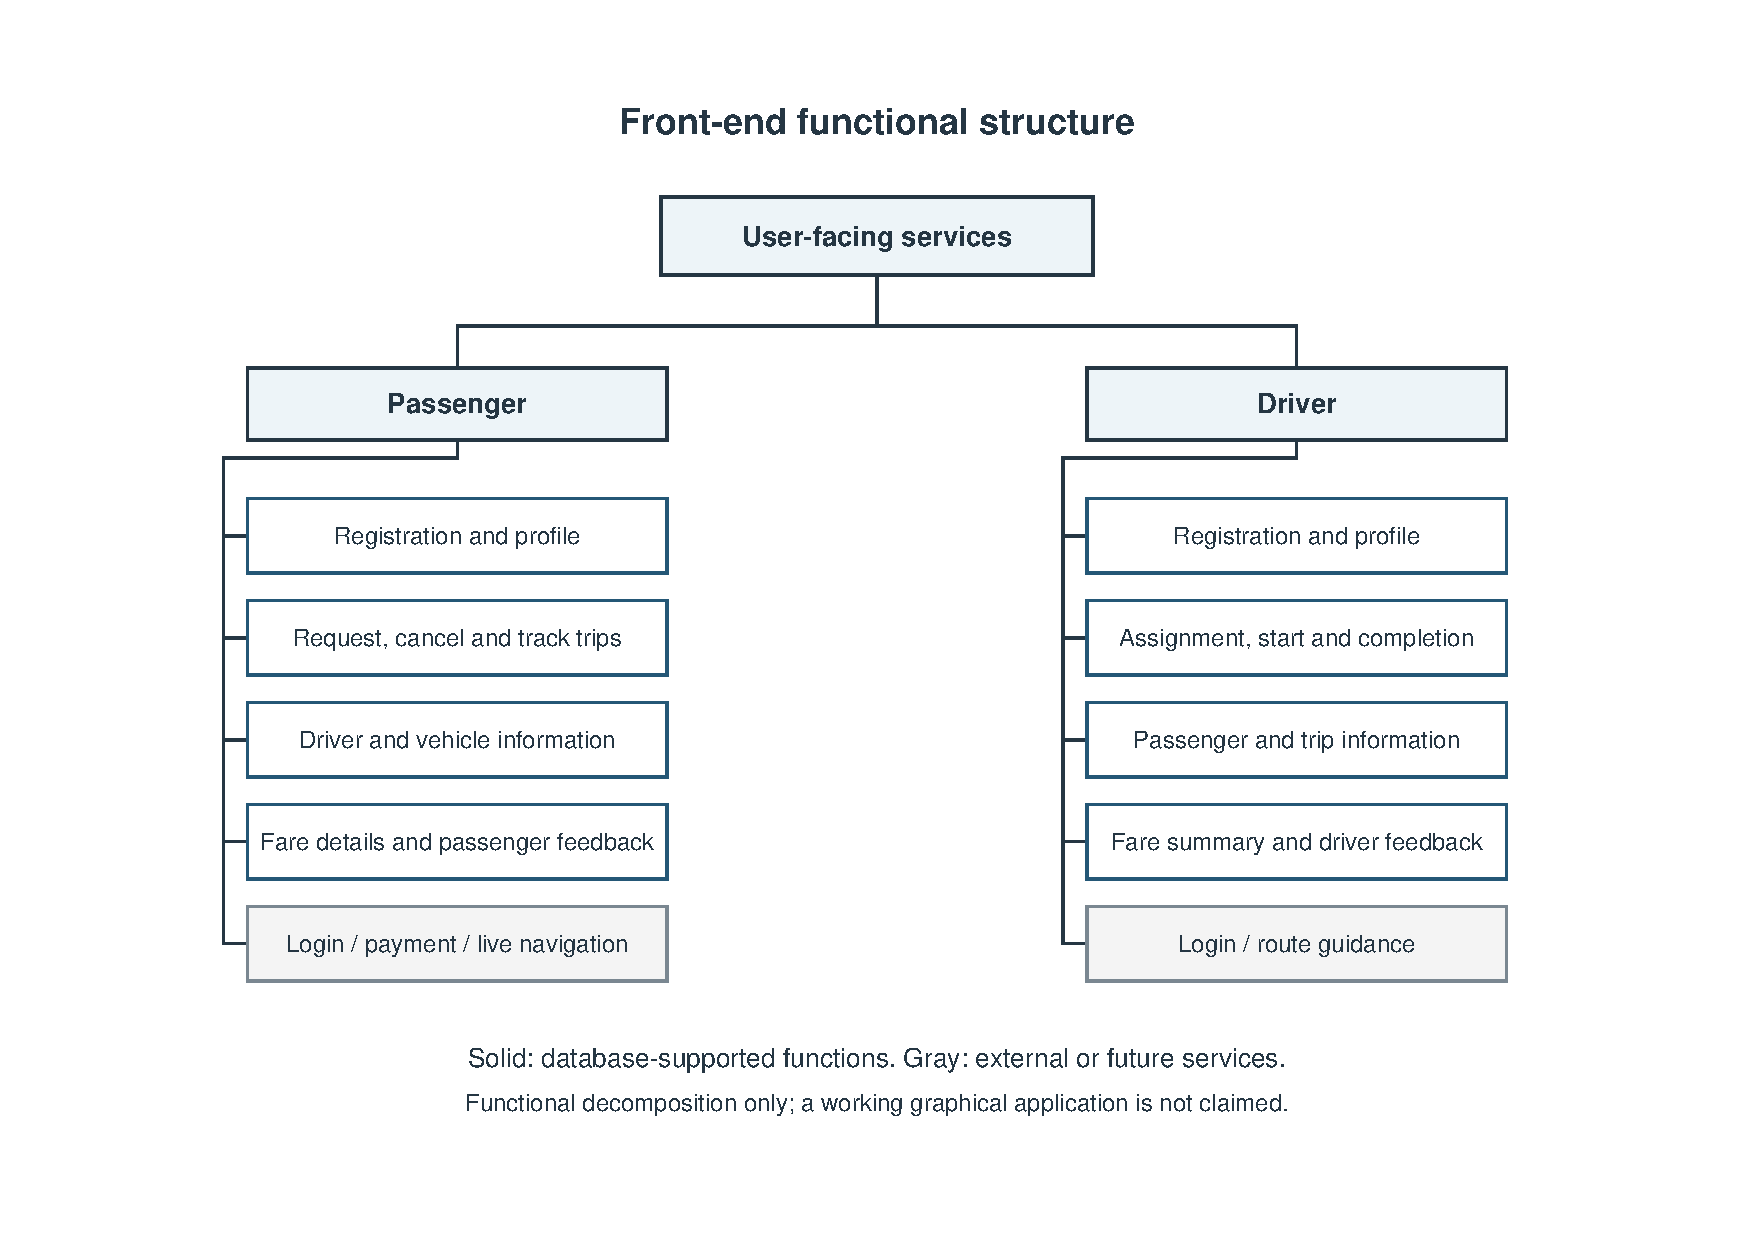
\includepdf[pages=1,fitpaper=true,pagecommand={\thispagestyle{empty}}]{figures/01_frontend.pdf}
\clearpage
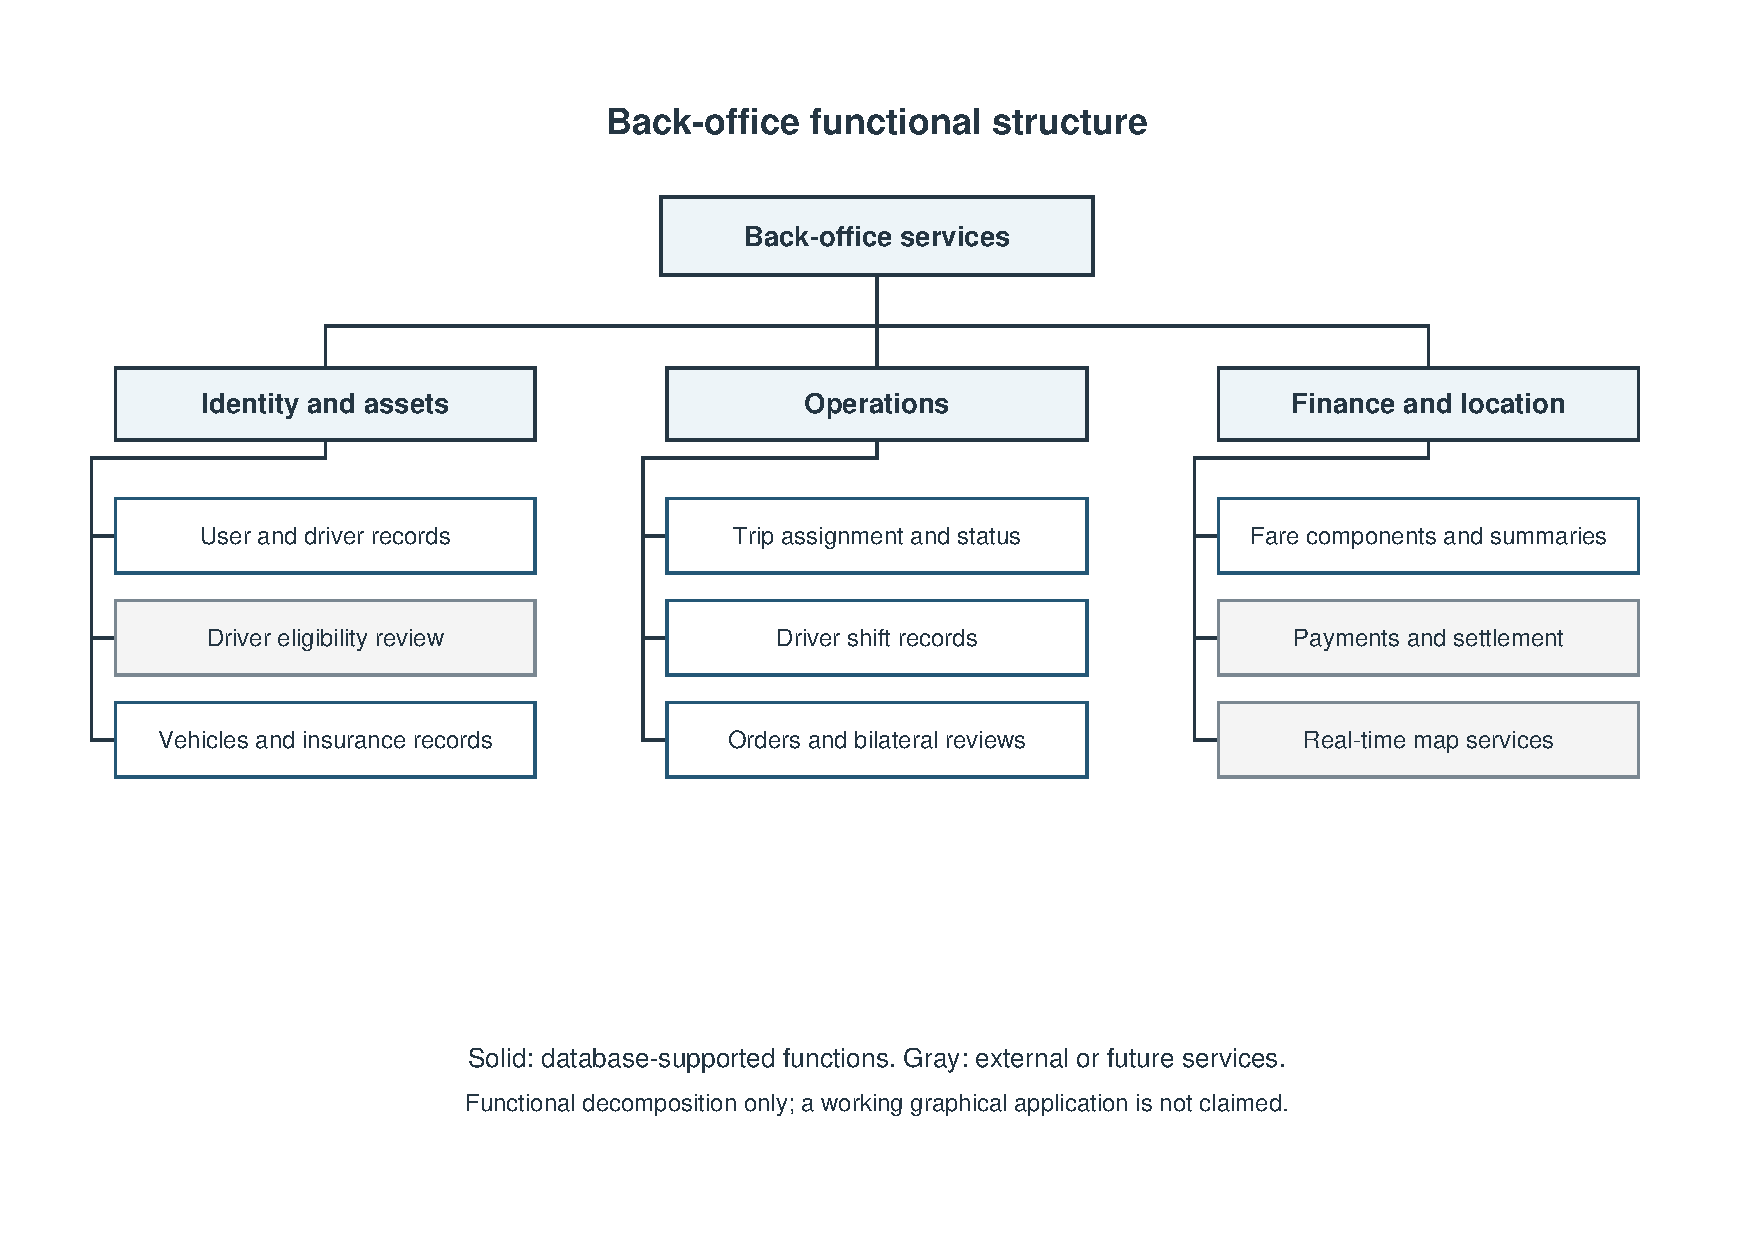
\includepdf[pages=1,fitpaper=true,pagecommand={\thispagestyle{empty}}]{figures/02_backend.pdf}

\clearpage
\section{Conceptual Design}
\subsection{Complete ER/EER model}
The following full-size plate uses the notation taught in LN3 and LN4. Entities are rectangles, attributes are ellipses, identifiers are underlined, relationships are diamonds, and minimum/maximum cardinalities are shown with circles, bars and crow feet. DriverShift, Review and Surcharge are identification-dependent entities and use double rectangles. Double diamonds make their identifying relationships explicit; LN3 notes that the distinction between ordinary and identifying relationship diamonds is not compulsory in the course.

The two specialization circles are marked o for overlapping user roles and d for disjoint trip outcomes. A single line from the supertype denotes partial specialization. Subtypes inherit the parent identifier; it is not repeated as a separate oval. The partial identifier shift\_\allowbreak{}start has a dashed underline. DriverShift is identified jointly by its driver and that start time. Review and Surcharge have no additional partial identifier because each completed trip has at most one of each.

All non-inherited conceptual attributes are shown. Foreign-key columns introduced by relational mapping are shown in the separate relational diagram, rather than duplicated as conceptual attributes. InsurancePolicy has its own globally unique identifier and is not treated as a weak entity. Lines that cross without a junction dot do not create an additional relationship.

\par\begingroup\small\noindent
\begin{tabularx}{\linewidth}{YY}
\toprule
Symbol & Meaning\\\midrule
Rectangle / double rectangle & Regular entity / identification-dependent entity\\
Ellipse / underline & Attribute / entity identifier\\
Dashed underline & Partial identifier within an owner\\
Diamond / double diamond & Relationship / identifying relationship\\
Circle + bar; two bars & Zero or one; exactly one\\
Circle + crow foot & Zero or many\\
o / d in a circle & Overlapping / disjoint specialization\\
Single supertype connector & Partial specialization\\
\bottomrule
\end{tabularx}
\par\endgroup
\clearpage
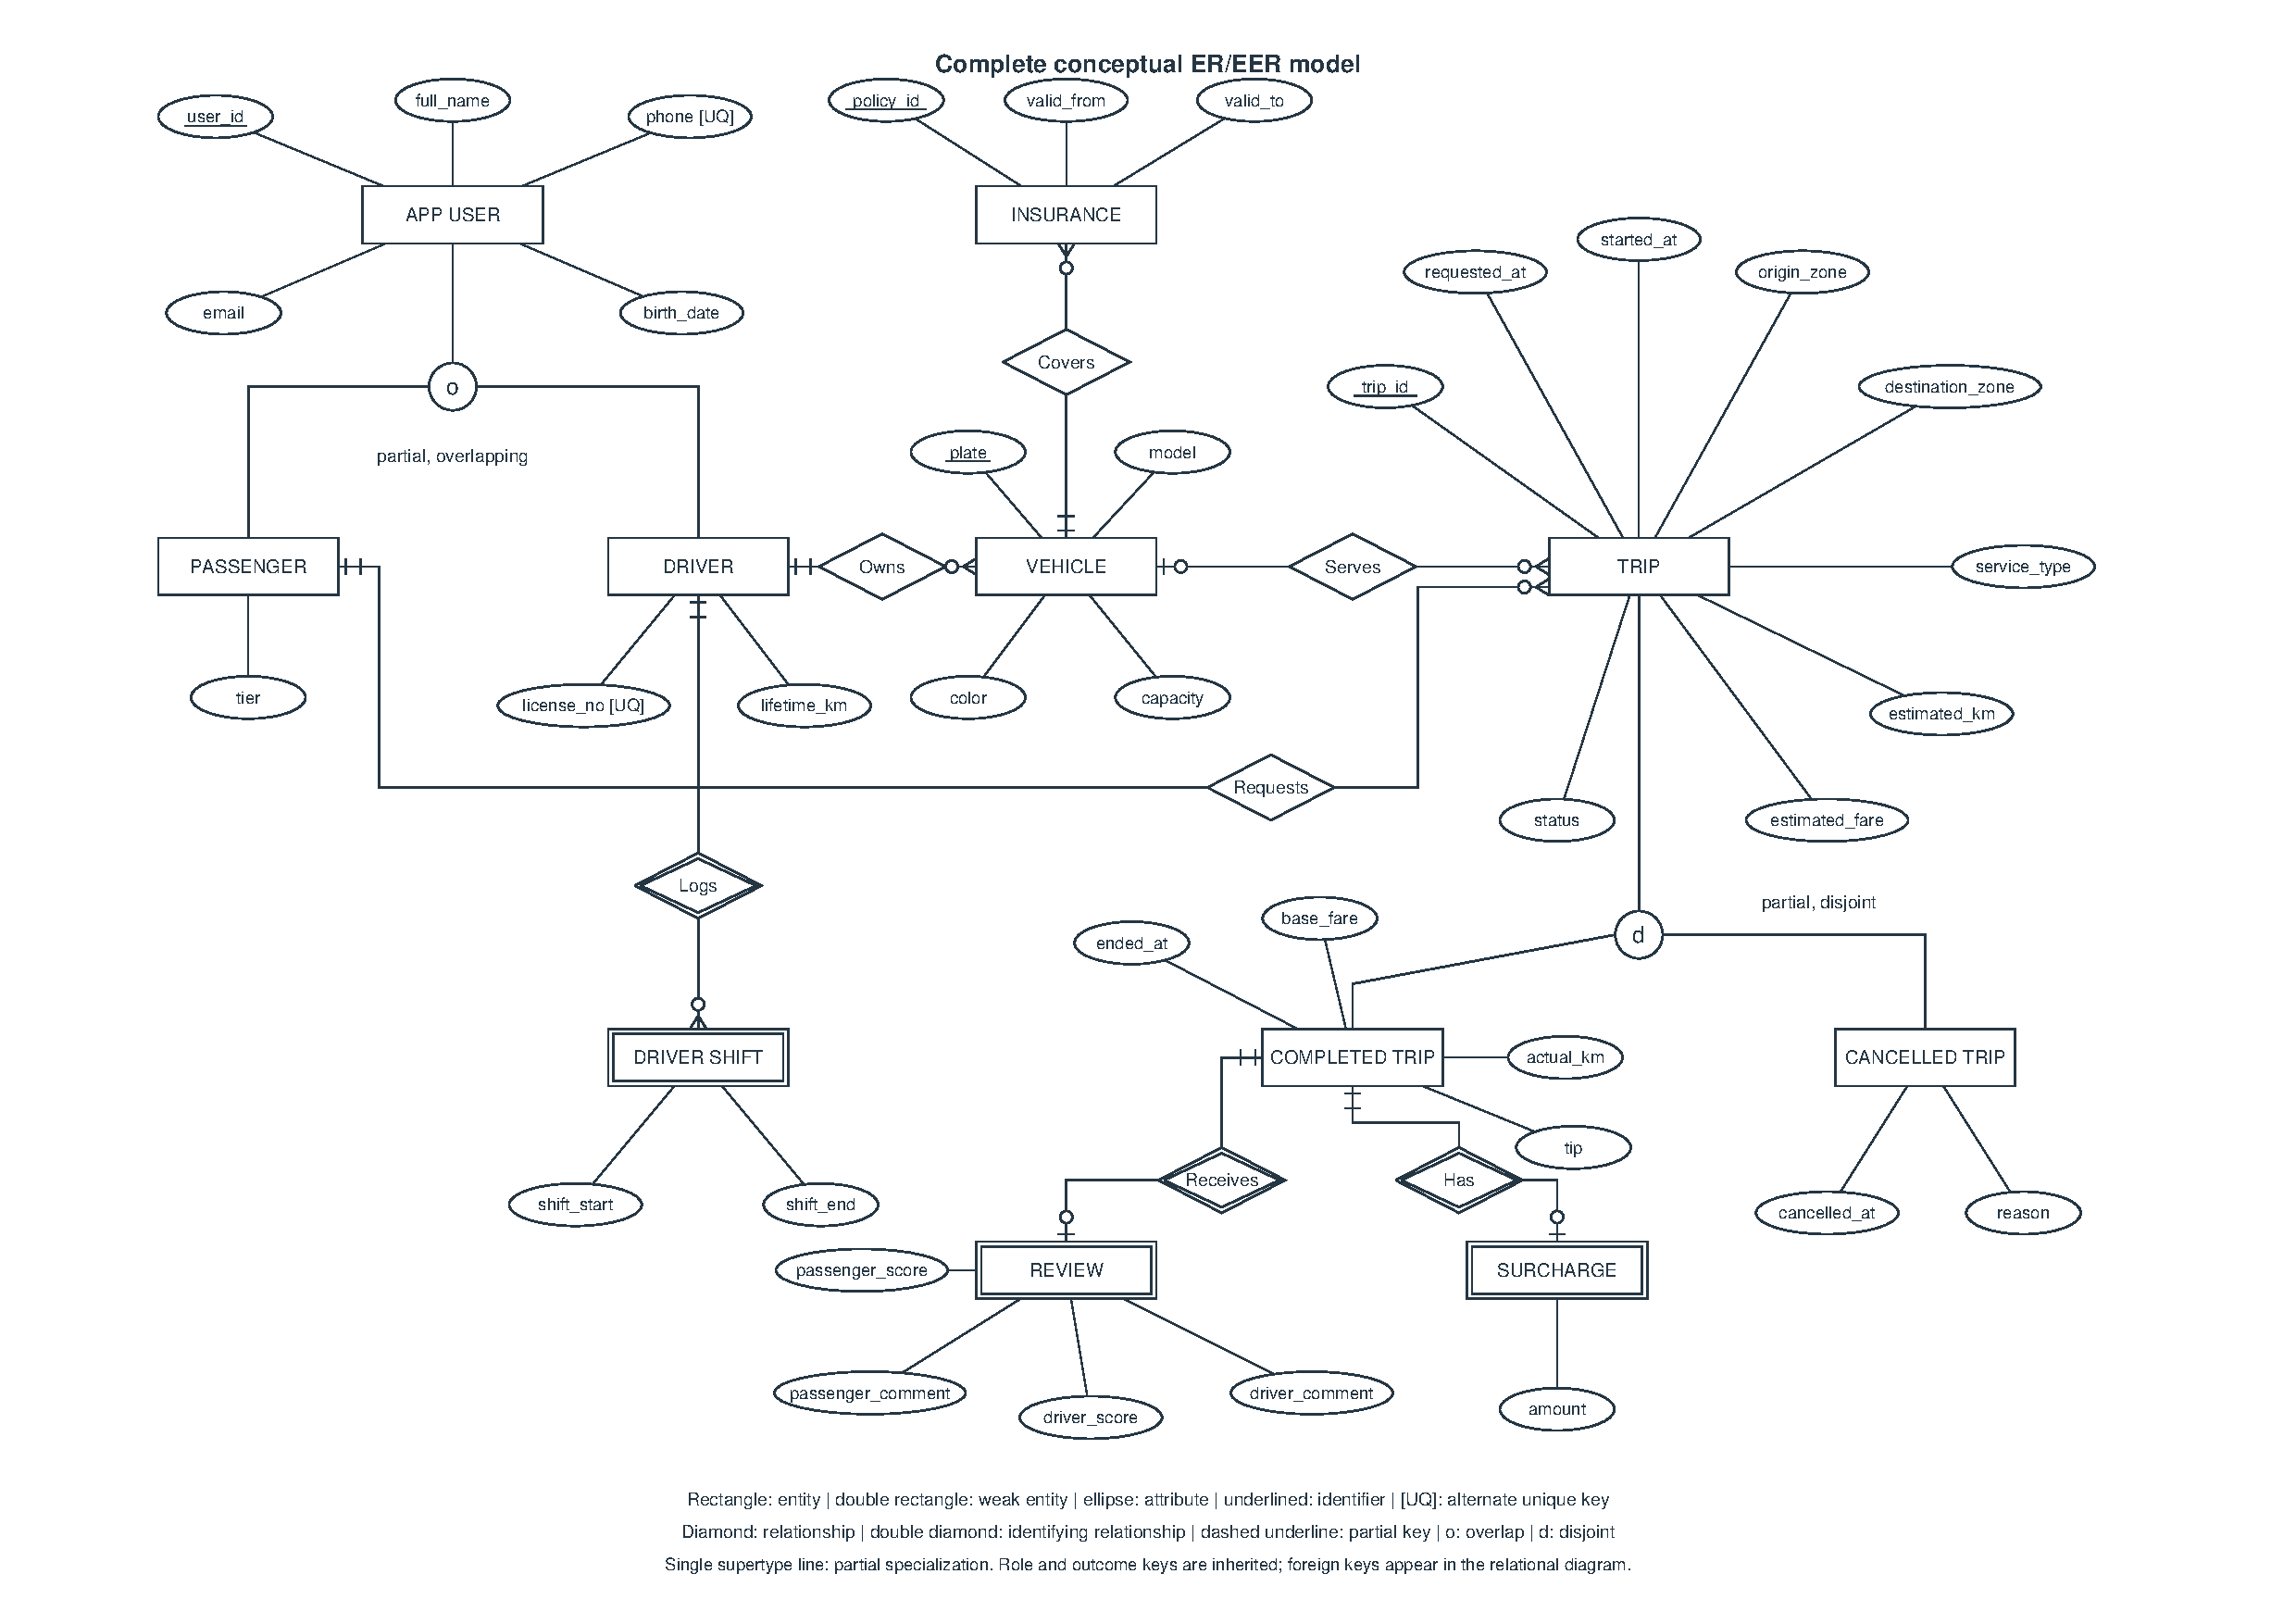
\includepdf[pages=1,fitpaper=true,pagecommand={\thispagestyle{empty}}]{figures/03_chen_eer.pdf}

\subsection{Relationships, participation and lifecycle}
Read the table as follows: for A → B, column two gives the number of B instances per A, and column three gives the number of A instances per B. A minimum of zero is optional participation; a minimum of one is mandatory participation. The outcome entities are additionally subject to the disjointness and state rules below.

A driver-to-trip association is derivable through Vehicle. It is not stored a second time. For example, if DEMO001 belongs to driver 1, any trip assigned DEMO001 is served by driver 1 within the fixed-ownership assumption. A driver with DEMO001 and another vehicle can therefore be associated with many trips without losing which vehicle served each one.

The design contains several one-to-many and optional one-to-one associations. A many-to-many association is not added simply to demonstrate a notation. If the scope later permits driver/vehicle reassignment over time, an assignment-history entity will become necessary, and the current fixed-ownership dependency must be revised.

\par\begingroup\small\noindent
\begin{tabularx}{\linewidth}{p{4.3cm}p{1.3cm}p{1.3cm}X}
\toprule
A → B & B per A & A per B & Rule\\\midrule
AppUser → Passenger & 0..1 & 1 & Partial overlapping specialization\\
AppUser → Driver & 0..1 & 1 & Same person can hold both roles\\
Driver → Vehicle & 0..N & 1 & Owner fixed during observation\\
Vehicle → InsurancePolicy & 0..N & 1 & Multiple policies/history allowed\\
Driver → DriverShift & 0..N & 1 & Start time is a partial identifier\\
Passenger → Trip & 0..N & 1 & One account requests each trip\\
Vehicle → Trip & 0..N & 0..1 & Required after assignment\\
Trip → CompletedTrip & 0..1 & 1 & Only completed outcome\\
Trip → CancelledTrip & 0..1 & 1 & Only cancelled outcome\\
CompletedTrip → Review & 0..1 & 1 & One row may contain both scores\\
CompletedTrip → Surcharge & 0..1 & 1 & Absent row means zero surcharge\\
\bottomrule
\end{tabularx}
\par\endgroup

The AppUser specialization is partial and overlapping: an identity can have neither role, either role, or both. Passenger and Driver inherit user\_\allowbreak{}id as both primary and foreign key. Shared contact attributes remain in AppUser.

Trip outcomes form a partial, disjoint specialization. An unfinished trip has no terminal detail. A COMPLETED trip has exactly one CompletedTrip and no CancelledTrip; a CANCELLED trip has exactly one CancelledTrip and no CompletedTrip. The implementation uses a status discriminator plus transaction-controlled detail creation.

Cancellation is allowed before a trip starts. Once IN\_\allowbreak{}PROGRESS, this simplified lifecycle only permits completion; emergency termination and partial-service refunds are outside scope. REQUESTED requires no vehicle and no start time. ASSIGNED requires a vehicle but no start time. IN\_\allowbreak{}PROGRESS and COMPLETED require both. CANCELLED may retain the previously assigned vehicle, but has no start time.


\begin{center}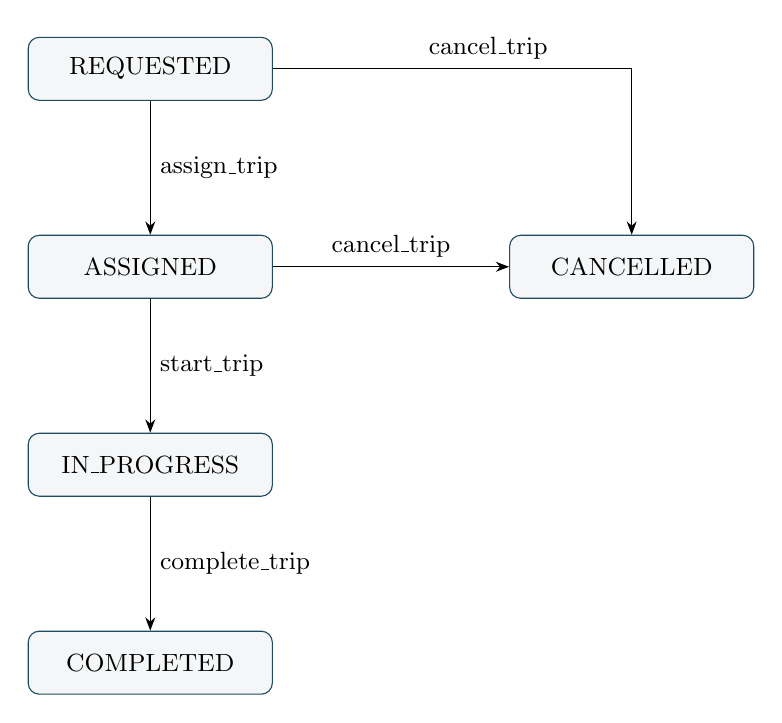
\begin{tikzpicture}[node distance=1.7cm,>=Stealth,every node/.style={font=\small},state/.style={draw=accent,rounded corners,fill=accent!5,minimum width=3.1cm,minimum height=.8cm}]
\node[state](a){REQUESTED};\node[state,below=of a](b){ASSIGNED};\node[state,below=of b](c){IN\_PROGRESS};\node[state,below=of c](d){COMPLETED};\node[state,right=3cm of b](x){CANCELLED};
\draw[->](a)--node[right]{assign\_trip}(b);\draw[->](b)--node[right]{start\_trip}(c);\draw[->](c)--node[right]{complete\_trip}(d);\draw[->](a.east)-|node[above,pos=.3]{cancel\_trip}(x.north);\draw[->](b)--node[above]{cancel\_trip}(x);
\end{tikzpicture}\end{center}
\begin{equation*}
\begin{gathered}{}[status=COMPLETED]\iff[\exists!\ CompletedTrip],\\
[status=CANCELLED]\iff[\exists!\ CancelledTrip].\end{gathered}
\end{equation*}
\clearpage
\section{Relational Mapping and Step-by-Step Normalization}
\begingroup\setlength{\parskip}{4pt}\renewcommand{\arraystretch}{1.1}\lstset{aboveskip=5pt,belowskip=5pt}
\subsection{From the ER/EER diagram to initial relations}
This chapter makes the design process explicit: map entities and relationships, write a provisional relational schema, inspect 1NF, remove partial dependencies for 2NF, remove transitive dependencies for 3NF, and then check every remaining determinant for BCNF. Each stage states what changes and what stays unchanged.

The starting schema below is a reconstructed design-stage worksheet used to explain the derivation. It is not a claim that these intermediate tables were executed in MySQL or copied verbatim from an earlier file. The actual database contains only the final schema. The worksheet retains the assigned driver in Trip0 alongside the vehicle, reflecting the original driver-to-trip association. The other entity mappings are kept intact. The 2NF section separately uses a clearly labeled counterexample to explain why driver descriptors should remain outside the shift relation; that counterexample is not an additional project table.

\par\begingroup\small\noindent
\begin{tabularx}{\linewidth}{p{3.3cm}X}
\toprule
Diagram construct & Initial relational mapping\\\midrule
Regular entities and attributes & One relation per entity; atomic attributes become columns. AppUser, Driver, Vehicle and InsurancePolicy retain their own identifiers.\\
User-role specialization & Passenger and Driver inherit the user key as PK/FK. Overlapping roles do not duplicate shared contact attributes.\\
Owns, Requests, Covers, Serves & Place the one-side key on the many side. Vehicle gets driver\_\allowbreak{}id; Trip gets passenger\_\allowbreak{}id and optional plate; InsurancePolicy gets plate.\\
Identifying relationships & Shift uses (driver\_\allowbreak{}id, shift\_\allowbreak{}start). Review and Surcharge inherit the completed-trip key.\\
Trip-outcome specialization & CompletedTrip and CancelledTrip inherit trip\_\allowbreak{}id. Disjointness and status consistency are additional integrity rules.\\
\bottomrule
\end{tabularx}
\par\endgroup
For example, a literal relationship relation Owns(driver\_\allowbreak{}id, plate) has plate as its key because each vehicle has one owner. It can be absorbed into Vehicle by adding driver\_\allowbreak{}id. Requests(passenger\_\allowbreak{}id, trip\_\allowbreak{}id) similarly places passenger\_\allowbreak{}id in Trip; Covers(plate, policy\_\allowbreak{}id) places plate in InsurancePolicy. Serves(plate, trip\_\allowbreak{}id) supplies the optional Trip.plate. These are cardinality-based mapping choices, not separate normalization steps. There is no many-to-many relationship requiring an extra bridge table in this scope.

\clearpage
\subsubsection*{Initial schema S0: relations before normalization}
\begingroup\small\renewcommand{\arraystretch}{1.12}\begin{longtable}{p{3.1cm}p{12.1cm}}\toprule
Initial relation & Attributes and candidate keys\\\midrule\endhead
app\_\allowbreak{}user & user\_\allowbreak{}id, full\_\allowbreak{}name, phone, email, birth\_\allowbreak{}date; Key(s): user\_\allowbreak{}id; alternate: phone\\[4pt]
passenger & passenger\_\allowbreak{}id, tier; Key(s): passenger\_\allowbreak{}id\\[4pt]
driver & driver\_\allowbreak{}id, license\_\allowbreak{}no, lifetime\_\allowbreak{}km; Key(s): driver\_\allowbreak{}id; alternate: license\_\allowbreak{}no\\[4pt]
vehicle & plate, driver\_\allowbreak{}id, model, color, capacity; Key(s): plate\\[4pt]
insurance\_\allowbreak{}policy & policy\_\allowbreak{}id, plate, valid\_\allowbreak{}from, valid\_\allowbreak{}to; Key(s): policy\_\allowbreak{}id\\[4pt]
driver\_\allowbreak{}shift & driver\_\allowbreak{}id, shift\_\allowbreak{}start, shift\_\allowbreak{}end; Key(s): (driver\_\allowbreak{}id, shift\_\allowbreak{}start)\\[4pt]
Trip0 & trip\_\allowbreak{}id, passenger\_\allowbreak{}id, plate, requested\_\allowbreak{}at, started\_\allowbreak{}at, origin\_\allowbreak{}zone, destination\_\allowbreak{}zone, service\_\allowbreak{}type, estimated\_\allowbreak{}km, estimated\_\allowbreak{}fare, status, driver\_\allowbreak{}id; Key(s): trip\_\allowbreak{}id\\[4pt]
completed\_\allowbreak{}trip & trip\_\allowbreak{}id, ended\_\allowbreak{}at, base\_\allowbreak{}fare, tip, actual\_\allowbreak{}km; Key(s): trip\_\allowbreak{}id\\[4pt]
cancelled\_\allowbreak{}trip & trip\_\allowbreak{}id, cancelled\_\allowbreak{}at, reason; Key(s): trip\_\allowbreak{}id\\[4pt]
review & trip\_\allowbreak{}id, passenger\_\allowbreak{}score, passenger\_\allowbreak{}comment, driver\_\allowbreak{}score, driver\_\allowbreak{}comment; Key(s): trip\_\allowbreak{}id\\[4pt]
surcharge & trip\_\allowbreak{}id, amount; Key(s): trip\_\allowbreak{}id\\[4pt]\bottomrule\end{longtable}\endgroup
DriverShift keeps only the driver key and the shift timestamps; driver descriptors remain in Driver. Trip0.driver\_\allowbreak{}id is the driver of the assigned plate and is absent when there is no assignment. All other relations already use the attributes and identifiers of the final entity mapping. Thus the normal-form checks can distinguish an actual necessary change from relations that already meet the criteria.

\subsection{First normal form: scalar values and a valid key}
1NF requires each attribute value to belong to its atomic domain rather than contain a repeating group. S0 passes this check: one row describes one user, vehicle, policy, shift or trip; phone is one registered phone value; each timestamp is one DATETIME value. A driver with two vehicles is represented by two Vehicle rows, not a comma-separated vehicle list. Multiple shifts are represented by multiple DriverShift rows.

Therefore S1 = S0: no relation is split merely to claim a 1NF transformation. Correcting the shift identifier is a separate key-design issue. A date alone, even combined with driver\_\allowbreak{}id, cannot identify two shifts by the same driver on one date. The mapping uses the actual start timestamp from the outset.

\par\begingroup\small\noindent
\begin{tabularx}{\linewidth}{YYY}
\toprule
driver\_\allowbreak{}id & shift\_\allowbreak{}start & shift\_\allowbreak{}end\\\midrule
1 & 2026-10-01 06:00:00 & 2026-10-01 13:00:00\\
1 & 2026-10-01 14:00:00 & 2026-10-01 23:00:00\\
\bottomrule
\end{tabularx}
\par\endgroup
These two rows come from the executed sample data. Both have the same driver and calendar date, but different shift\_\allowbreak{}start values. Atomicity and uniqueness are related design checks; changing a deficient key alone is not a 1NF decomposition.

\subsection{Second normal form: inspect composite-key dependencies}
2NF requires 1NF and requires every non-prime attribute to depend on each candidate key in full. DriverShift is the only S1 relation with a composite candidate key. Its key is (driver\_\allowbreak{}id, shift\_\allowbreak{}start), and its only non-prime attribute is shift\_\allowbreak{}end. A driver has many shifts, and different drivers may start at the same time. Neither component alone determines shift\_\allowbreak{}end; the complete pair does.

Every other S1 relation has only single-attribute candidate keys. Under the stated dependencies, none can exhibit a partial dependency on a nonempty proper subset of a key. Therefore S2 = S1: the mapped schema is already in 2NF. Keeping a table unchanged after a successful check is part of the normalization process, rather than a missing transformation.

\begin{lstlisting}
DriverShift(driver_id, shift_start, shift_end)
Candidate key: (driver_id, shift_start)
(driver_id, shift_start) -> shift_end
Neither driver_id nor shift_start alone determines shift_end.
Decision: retain DriverShift unchanged in S2.
\end{lstlisting}
\subsubsection*{Counterexample: what would break 2NF?}
For comparison, suppose a convenience worksheet copied Driver's license\_\allowbreak{}no and lifetime\_\allowbreak{}km into each shift. Call it ShiftWide. This is an illustrative joined view of the existing sample records, not the actual initial schema and not a table that was implemented. Because license\_\allowbreak{}no is unique and mandatory, its candidate keys would be (driver\_\allowbreak{}id, shift\_\allowbreak{}start) and (license\_\allowbreak{}no, shift\_\allowbreak{}start).

In ShiftWide, the non-prime lifetime\_\allowbreak{}km depends on driver\_\allowbreak{}id alone and on license\_\allowbreak{}no alone. Both are proper subsets of candidate keys, so this counterexample violates 2NF. License\_\allowbreak{}no itself is prime because it belongs to an alternative candidate key; the decisive 2NF violation is the non-prime mileage attribute.

\begin{lstlisting}
Counterexample only:
ShiftWide(driver_id, shift_start, shift_end, license_no, lifetime_km)
driver_id -> license_no, lifetime_km
license_no -> driver_id, lifetime_km

Its correction would be:
Driver(driver_id, license_no, lifetime_km)
DriverShift(driver_id, shift_start, shift_end)
These are already the two relations in the mapped schema.
\end{lstlisting}
\par\begingroup\small\noindent
\begin{tabularx}{\linewidth}{YYYY}
\toprule
driver\_\allowbreak{}id & shift\_\allowbreak{}start & license\_\allowbreak{}no & lifetime\_\allowbreak{}km\\\midrule
1 & 2026-10-01 06:00:00 & DEMO-LIC-001 & 1125.00\\
1 & 2026-10-01 14:00:00 & DEMO-LIC-001 & 1125.00\\
\bottomrule
\end{tabularx}
\par\endgroup
The two reconstructed ShiftWide rows repeat the same registered mileage; a correction would have to update several shift rows. Separating Driver from DriverShift prevents that anomaly and permits a driver to exist before any shift is logged.

The illustrative decomposition is lossless because the intersection, driver\_\allowbreak{}id, determines all Driver attributes. Joining the projections on driver\_\allowbreak{}id reconstructs the original shift rows. Each listed dependency can be checked in one resulting relation, so it preserves the dependency set. The final schema already has this separation and a foreign key for the owner; no extra physical table or artificial 2NF split is needed.

\subsection{Third normal form, BCNF and the final schema}
For every non-trivial dependency X -> A, 3NF requires X to be a superkey or A to be prime. In the assigned-trip part of Trip0, trip\_\allowbreak{}id determines plate and fixed vehicle ownership gives plate -> driver\_\allowbreak{}id. Plate is not a superkey of Trip0 because the same vehicle can serve several trips; driver\_\allowbreak{}id is not a prime attribute. The dependency therefore violates 3NF, even though Trip0 has already passed 2NF.

\begin{lstlisting}
Trip0(trip_id, passenger_id, plate, ..., status, driver_id)
trip_id -> plate
plate -> driver_id
Therefore: trip_id -> plate -> driver_id

Project into:
Trip(trip_id, passenger_id, plate, ..., status)
VehicleOwner(plate, driver_id)

VehicleOwner is already represented inside:
Vehicle(plate, driver_id, model, color, capacity)
\end{lstlisting}
Remove driver\_\allowbreak{}id from Trip0 and use the existing Vehicle relation to determine the driver. For example, sample trip 1 uses DEMO001, and Vehicle assigns DEMO001 to driver 1. A duplicated Trip0.driver\_\allowbreak{}id of 2 would contradict that fact; the final schema cannot store that contradictory duplicate. The dispatch procedure still accepts both identifiers and verifies their match.

For assigned trips, the decomposition is lossless because the intersection {plate} determines VehicleOwner. The dependency trip\_\allowbreak{}id -> plate remains in Trip, plate -> driver\_\allowbreak{}id remains in Vehicle, and their transitive implication is preserved across the design. The conceptual proof concerns assigned records with a present vehicle. Unassigned requests have no vehicle-owner association; in the SQL representation their plate is NULL. A LEFT JOIN retains those requests with a NULL derived driver. It would be incorrect to claim that an INNER JOIN preserves unassigned rows or to apply the classical no-NULL proof to them unchanged.

BCNF strengthens the determinant condition: every non-trivial determinant must be a superkey, even when the dependent attribute is prime. Driver satisfies it because both driver\_\allowbreak{}id and license\_\allowbreak{}no are candidate keys. AppUser similarly has user\_\allowbreak{}id and phone. In DriverShift, the only stated non-trivial determinant is the complete pair (driver\_\allowbreak{}id, shift\_\allowbreak{}start). The remaining final relations have only their candidate-key dependencies under the stated assumptions. No further BCNF split is required after S3. The following table checks every final relation.

\par\begingroup\small\noindent
\begin{tabularx}{\linewidth}{p{3.0cm}p{4.0cm}X}
\toprule
Relation & Candidate keys & Functional dependencies\\\midrule
app\_\allowbreak{}user & user\_\allowbreak{}id; phone & Either key → all other attributes\\
passenger & passenger\_\allowbreak{}id & passenger\_\allowbreak{}id → tier\\
driver & driver\_\allowbreak{}id; license\_\allowbreak{}no & Either key → all other attributes\\
vehicle & plate & plate → driver\_\allowbreak{}id, model, color, capacity\\
insurance\_\allowbreak{}policy & policy\_\allowbreak{}id & policy\_\allowbreak{}id → plate, valid\_\allowbreak{}from, valid\_\allowbreak{}to\\
driver\_\allowbreak{}shift & (driver\_\allowbreak{}id, shift\_\allowbreak{}start) & Composite key → shift\_\allowbreak{}end\\
trip & trip\_\allowbreak{}id & trip\_\allowbreak{}id → every remaining attribute\\
completed\_\allowbreak{}trip & trip\_\allowbreak{}id & trip\_\allowbreak{}id → ended\_\allowbreak{}at, base\_\allowbreak{}fare, tip, actual\_\allowbreak{}km\\
cancelled\_\allowbreak{}trip & trip\_\allowbreak{}id & trip\_\allowbreak{}id → cancelled\_\allowbreak{}at, reason\\
review & trip\_\allowbreak{}id & trip\_\allowbreak{}id → both scores and comments\\
surcharge & trip\_\allowbreak{}id & trip\_\allowbreak{}id → amount\\
\bottomrule
\end{tabularx}
\par\endgroup

There are no additional asserted dependencies such as model -> capacity or distance -> fare. Vehicle capacity is recorded per vehicle, and fare includes components not determined by distance alone. The normal-form conclusion follows from the declared business semantics; a small dataset cannot establish all real-world functional dependencies.

Some changes are not normal-form decompositions. Separating CompletedTrip from CancelledTrip expresses disjoint outcomes. Keeping Surcharge separate expresses an optional one-to-one detail: merging its amount into CompletedTrip would not, by itself, violate BCNF. Giving Review one trip\_\allowbreak{}id key enforces at most one bilateral review row per completed trip; an independent review\_\allowbreak{}id plus UNIQUE(trip\_\allowbreak{}id) could also be normalized. These choices should not be presented as necessary steps from 2NF to 3NF.

\par\begingroup\small\noindent
\begin{tabularx}{\linewidth}{p{2.5cm}p{6.2cm}X}
\toprule
Stage & Decision & Result\\\midrule
S0 → S1 & Atomic values; correct shift identifier & Already 1NF; no split\\
S1 → S2 & Check the composite DriverShift key & Already 2NF; no split\\
S2 → S3 & Remove plate -> driver\_\allowbreak{}id from Trip0 & Trip + existing Vehicle; 3NF\\
S3 → BCNF & Inspect all non-trivial determinants & No additional split; 11 final tables\\
\bottomrule
\end{tabularx}
\par\endgroup
The final relational diagram below shows all 11 operational tables and every implemented column. PK, FK and UQ identify primary, foreign and alternate keys; ? marks a nullable column. Its fields are generated from the executed MySQL data dictionary and match the SQL implementation that follows.

\clearpage
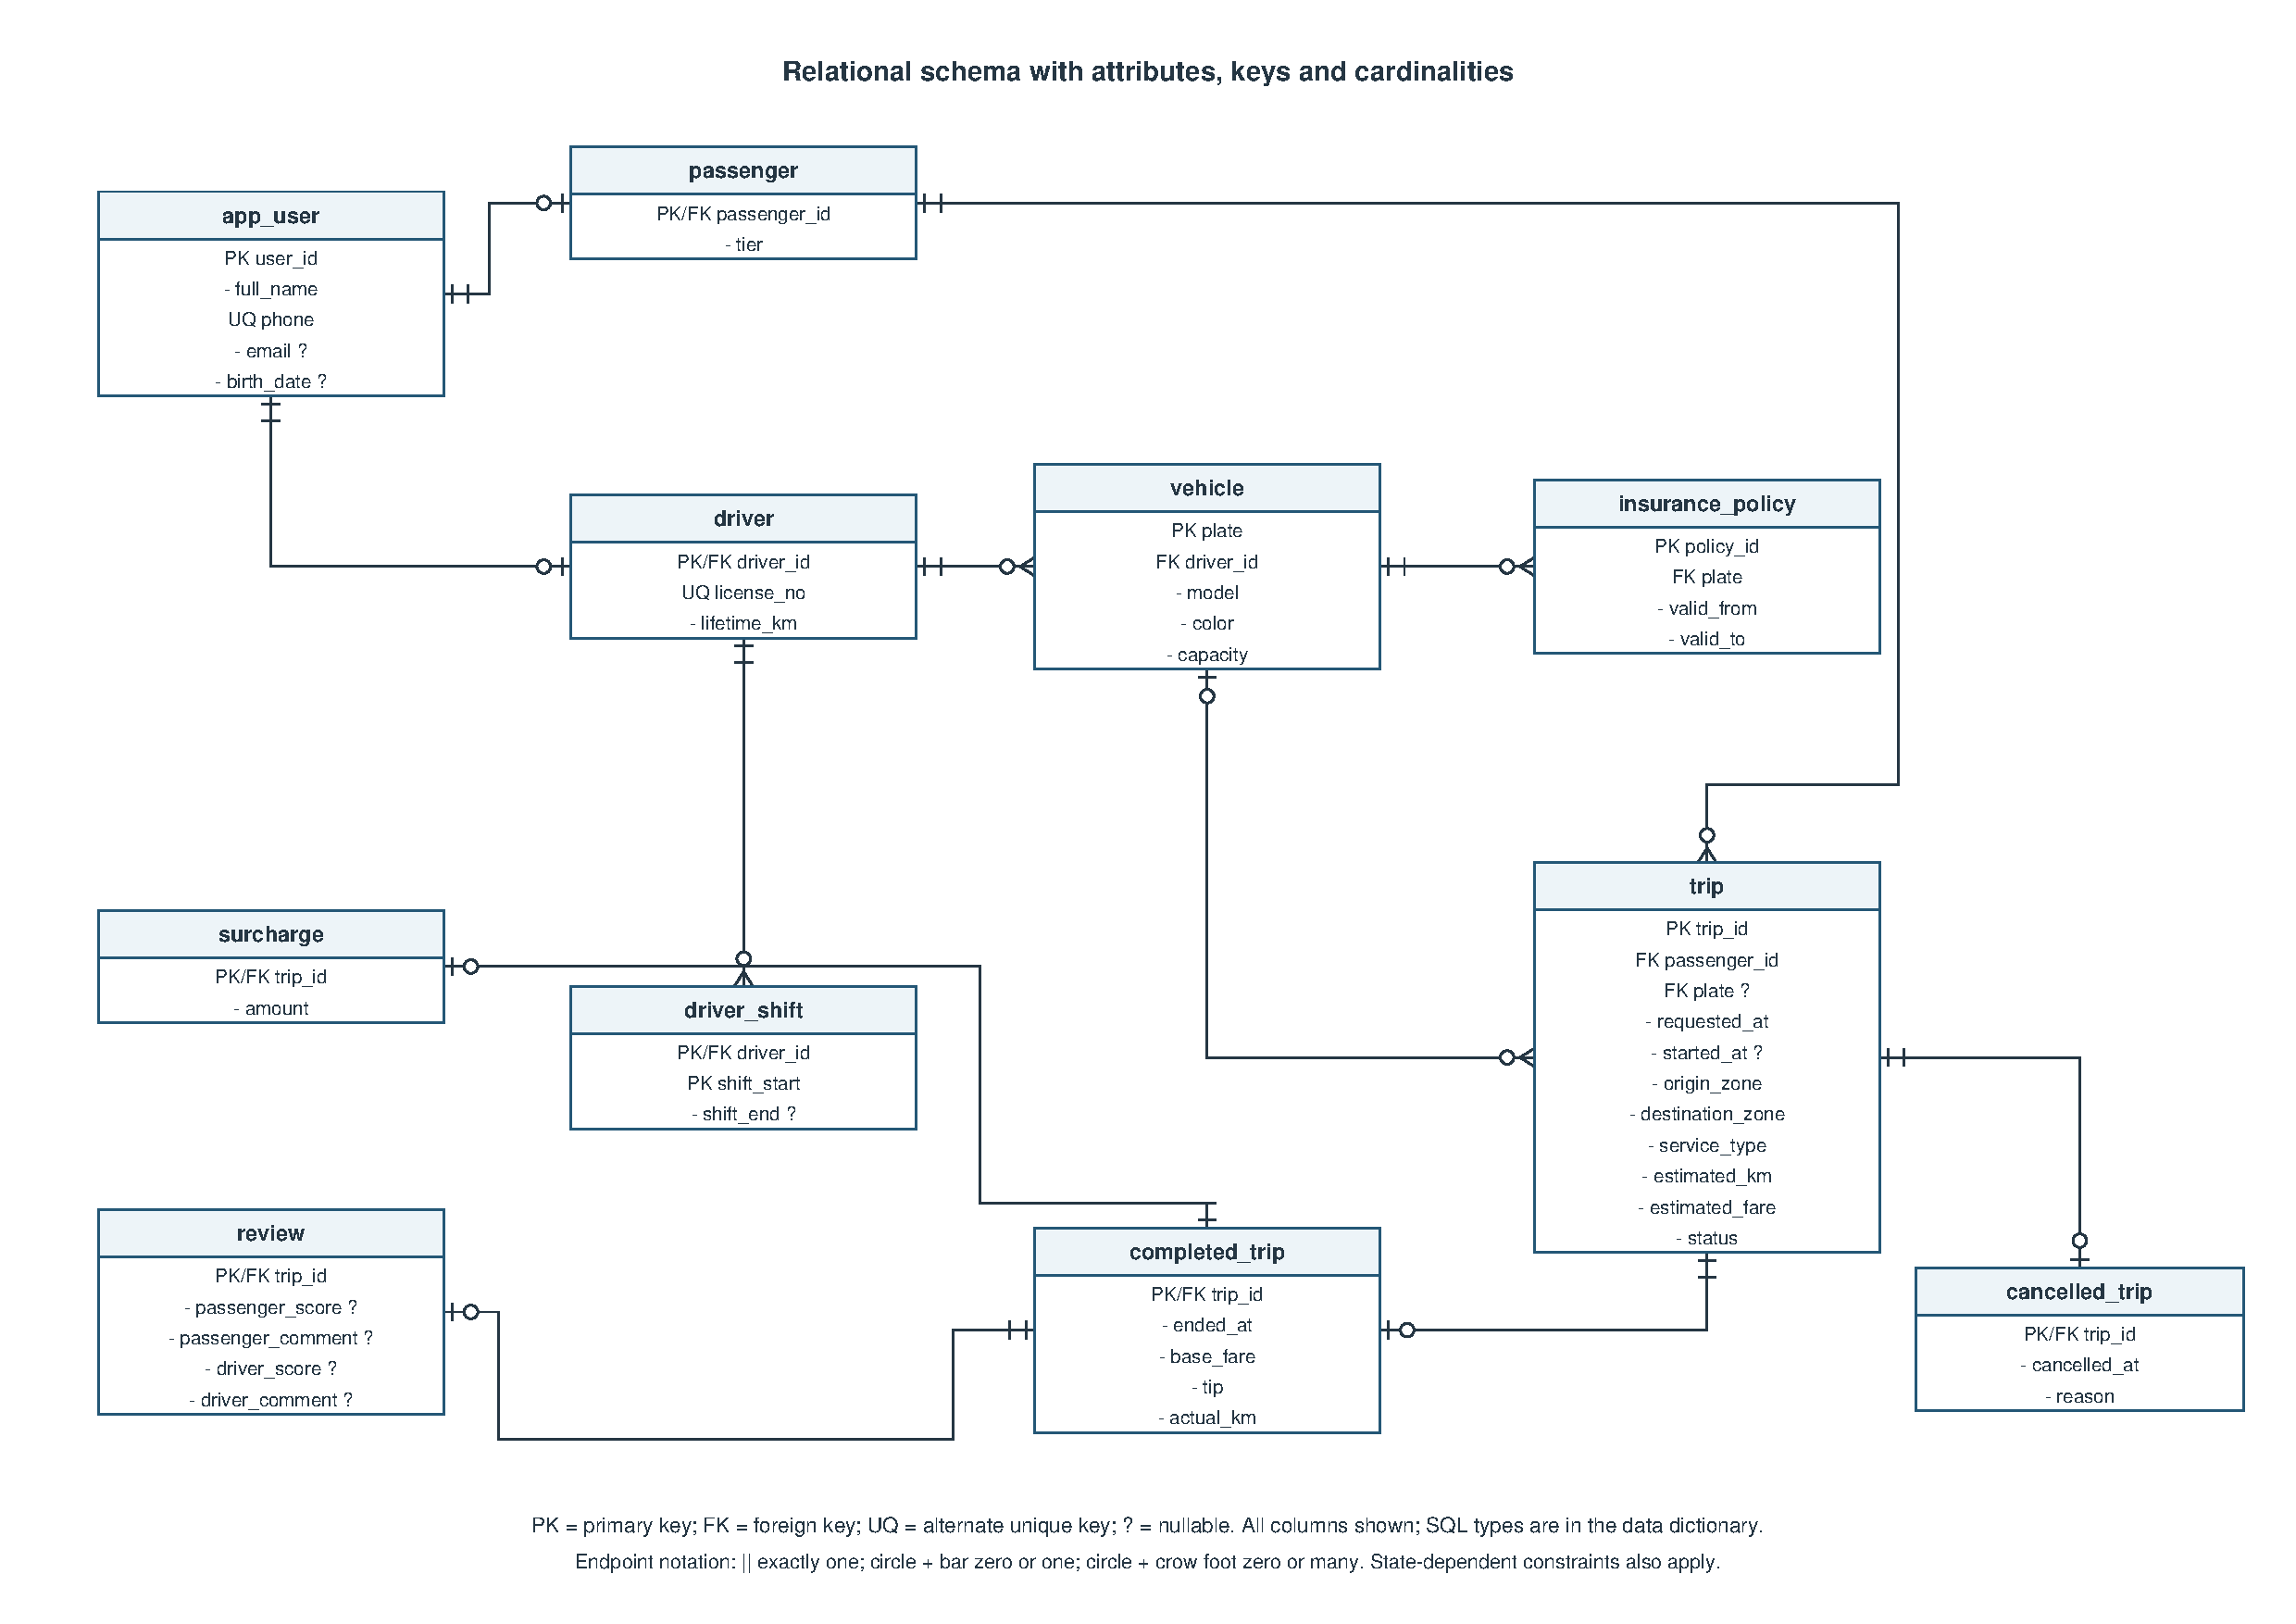
\includepdf[pages=1,fitpaper=true,pagecommand={\thispagestyle{empty}}]{figures/04_relational.pdf}
\endgroup
\clearpage
\section{Database Implementation and Validation}
\subsection{Physical tables, constraints and creation SQL}
The executed engine is MySQL 8.4.13. All operational tables use InnoDB. PRIMARY KEY and UNIQUE constraints protect entity identity; FOREIGN KEY constraints protect references; CHECK constraints enforce local domains and chronology. Referenced history is protected by the default restrictive deletion policy. There is no broad ON DELETE CASCADE from a user to completed service records.

The application role can create identities and registration records, insert only the permitted booking columns, submit or update reviews, read results, and execute lifecycle procedures. It cannot directly change Trip.status or insert/update outcome records. Procedure execution uses the definer's privileges. The disposable test account is removed after verification; the delivery does not ship a passwordless production account.

Guard triggers validate a completion's parent state and end time, validate a cancellation's parent state and time, and prevent vehicle-owner changes. Because ordinary MySQL CHECK expressions cannot express all cross-table invariants here, the lifecycle procedures enforce the complete state/detail change as one transaction. An administrator with direct write access can still bypass the intended workflow; the report's guarantee applies to the application interface and declared role.

Indexes include (passenger\_\allowbreak{}id, requested\_\allowbreak{}at) for passenger history and (status, requested\_\allowbreak{}at) for operational filtering. Primary and foreign-key indexes support joins. The saved EXPLAIN output documents the optimizer's actual choice on this small dataset; no production latency claim is made. In this run, the passenger-history query uses range access on ix\_\allowbreak{}trip\_\allowbreak{}passenger\_\allowbreak{}time with an estimate of 3 rows and Using index condition.

\begin{lstlisting}
CREATE VIEW trip_service AS
SELECT t.*, v.driver_id
FROM trip t LEFT JOIN vehicle v ON v.plate=t.plate;

-- A booking cannot directly choose status or completion detail
-- when inserted through the application role.
GRANT INSERT (trip_id, passenger_id, requested_at,
 origin_zone, destination_zone, service_type,
 estimated_km, estimated_fare)
ON ride_hailing.trip TO 'ride_hailing_app';
\end{lstlisting}

The following listing reproduces the complete executed DDL for the 11 operational tables. It includes the database declaration, primary and alternate keys, foreign keys, domain constraints and indexes. CREATE TABLE order follows parent-before-child dependencies, so foreign-key checks remain enabled during construction.

InnoDB provides transactional tables. The script intentionally fails if the schema already exists. No application data are silently deleted to make a demonstration pass. The complete procedure and trigger definitions remain in the companion SQL file; the lifecycle section explains how they are used.

\lstinputlisting[language=SQL,basicstyle=\ttfamily\footnotesize]{sql/01_schema.sql}
\subsection{Loaded data and executable SQL demonstrations}
The generator uses a local pseudorandom seed of 20261118. It creates 200 trips requested from 1 to 20 October 2026, with a predetermined mix of terminal and open states shuffled across the period. Timestamps are local Asia/Shanghai civil times stored as DATETIME; timezone conversion is not part of this single-region example.

The data includes one identity with both roles, one registered identity with neither role, multiple vehicles for selected drivers, and two shifts per driver per day. Completed trips include optional tips, optional surcharges and partial or bilateral feedback. Cancellation can occur before or after assignment. Open states intentionally exercise optional relationships.

All personal names, contact values, license numbers and vehicle identifiers are fabricated. The email domain example.invalid prevents them from resembling usable addresses. The generated state proportions and fees are input assumptions, not measured business performance. Stored driver lifetime\_\allowbreak{}km is a registration snapshot, not an aggregate maintained from these trips.

The reproduction sequence creates a new schema, loads routines, generates and imports synthetic records through the lifecycle interface, builds the analytical snapshot, creates the application role, then runs validation. Test fixtures use reserved identifiers and are removed before published outputs are collected. The generator seed and resulting counts are retained alongside the SQL and query results.

\par\begingroup\small\noindent
\begin{tabularx}{\linewidth}{YY}
\toprule
Operational table & Rows\\\midrule
app\_\allowbreak{}user & 34\\
passenger & 26\\
driver & 8\\
vehicle & 12\\
insurance\_\allowbreak{}policy & 12\\
driver\_\allowbreak{}shift & 320\\
trip & 200\\
completed\_\allowbreak{}trip & 130\\
cancelled\_\allowbreak{}trip & 30\\
review & 98\\
surcharge & 52\\
\bottomrule
\end{tabularx}
\par\endgroup

SHOW TABLES verifies which objects actually exist after the build. The output includes 11 operational tables, four dw\_\allowbreak{} analytical tables and two views. DESCRIBE trip provides a second, independent view of the implemented columns. The selected output columns below are Field, Type, Null and Key; the full raw output is supplied with the evidence files.

\noindent\begin{minipage}[t]{.29\linewidth}\vspace{0pt}\par\noindent\begin{minipage}{\linewidth}\setlength{\parskip}{0pt}\renewcommand{\arraystretch}{1.08}\titlespacing*{\subsection}{0pt}{7pt}{4pt}\lstset{aboveskip=4pt,belowskip=4pt}
\subsection*{show\_\allowbreak{}tables}
\begin{lstlisting}
SHOW TABLES;
\end{lstlisting}
\par\begingroup\small\noindent
\begin{tabularx}{\linewidth}{Y}
\toprule
Tables\_\allowbreak{}in\_\allowbreak{}ride\_\allowbreak{}hailing\\\midrule
app\_\allowbreak{}user\\
cancelled\_\allowbreak{}trip\\
completed\_\allowbreak{}trip\\
driver\\
driver\_\allowbreak{}shift\\
dw\_\allowbreak{}date\\
dw\_\allowbreak{}driver\\
dw\_\allowbreak{}trip\_\allowbreak{}fact\\
dw\_\allowbreak{}vehicle\\
insurance\_\allowbreak{}policy\\
passenger\\
review\\
surcharge\\
trip\\
trip\_\allowbreak{}financials\\
trip\_\allowbreak{}service\\
vehicle\\
\bottomrule
\end{tabularx}
\par\endgroup
\end{minipage}\par\vspace{5pt}
\end{minipage}\hfill\begin{minipage}[t]{.68\linewidth}\vspace{0pt}\par\noindent\begin{minipage}{\linewidth}\setlength{\parskip}{0pt}\renewcommand{\arraystretch}{1.08}\titlespacing*{\subsection}{0pt}{7pt}{4pt}\lstset{aboveskip=4pt,belowskip=4pt}
\subsection*{describe\_\allowbreak{}trip}
\begin{lstlisting}
DESCRIBE trip;
\end{lstlisting}
\par\begingroup\small\noindent
\begin{tabularx}{\linewidth}{YYYY}
\toprule
Field & Type & Null & Key\\\midrule
trip\_\allowbreak{}id & int & NO & PRI\\
passenger\_\allowbreak{}id & int & NO & MUL\\
plate & varchar(12) & YES & MUL\\
requested\_\allowbreak{}at & datetime & NO & \\
started\_\allowbreak{}at & datetime & YES & \\
origin\_\allowbreak{}zone & varchar(30) & NO & \\
destination\_\allowbreak{}zone & varchar(30) & NO & \\
service\_\allowbreak{}type & varchar(12) & NO & \\
estimated\_\allowbreak{}km & decimal(8,2) & NO & \\
estimated\_\allowbreak{}fare & decimal(10,2) & NO & \\
status & varchar(12) & NO & MUL\\
\bottomrule
\end{tabularx}
\par\endgroup
\end{minipage}\par\vspace{5pt}
\end{minipage}
\subsubsection*{Inserted data for users and roles}
These ordered SELECT queries show actual inserted rows. User 1 appears in both the passenger and driver tables, demonstrating overlapping specialization. The user sample shows selected identity columns; the complete column definitions remain in the data dictionary.

\par\noindent\begin{minipage}{\linewidth}\setlength{\parskip}{0pt}\renewcommand{\arraystretch}{1.08}\titlespacing*{\subsection}{0pt}{7pt}{4pt}\lstset{aboveskip=4pt,belowskip=4pt}
\subsection*{app\_\allowbreak{}user}
\begin{lstlisting}
SELECT user_id,full_name,phone
FROM app_user
ORDER BY user_id LIMIT 3;
\end{lstlisting}
\par\begingroup\small\noindent
\begin{tabularx}{\linewidth}{YYY}
\toprule
user\_\allowbreak{}id & full\_\allowbreak{}name & phone\\\midrule
1 & Demo User 1 & +860000000001\\
2 & Demo User 2 & +860000000002\\
3 & Demo User 3 & +860000000003\\
\bottomrule
\end{tabularx}
\par\endgroup
\end{minipage}\par\vspace{5pt}
\par\noindent\begin{minipage}{\linewidth}\setlength{\parskip}{0pt}\renewcommand{\arraystretch}{1.08}\titlespacing*{\subsection}{0pt}{7pt}{4pt}\lstset{aboveskip=4pt,belowskip=4pt}
\subsection*{passenger}
\begin{lstlisting}
SELECT *
FROM passenger
ORDER BY passenger_id LIMIT 3;
\end{lstlisting}
\par\begingroup\small\noindent
\begin{tabularx}{\linewidth}{YY}
\toprule
passenger\_\allowbreak{}id & tier\\\midrule
1 & PLATINUM\\
101 & STANDARD\\
102 & GOLD\\
\bottomrule
\end{tabularx}
\par\endgroup
\end{minipage}\par\vspace{5pt}
\par\noindent\begin{minipage}{\linewidth}\setlength{\parskip}{0pt}\renewcommand{\arraystretch}{1.08}\titlespacing*{\subsection}{0pt}{7pt}{4pt}\lstset{aboveskip=4pt,belowskip=4pt}
\subsection*{driver}
\begin{lstlisting}
SELECT *
FROM driver
ORDER BY driver_id LIMIT 3;
\end{lstlisting}
\par\begingroup\small\noindent
\begin{tabularx}{\linewidth}{YYY}
\toprule
driver\_\allowbreak{}id & license\_\allowbreak{}no & lifetime\_\allowbreak{}km\\\midrule
1 & DEMO-LIC-001 & 1125.00\\
2 & DEMO-LIC-002 & 1250.00\\
3 & DEMO-LIC-003 & 1375.00\\
\bottomrule
\end{tabularx}
\par\endgroup
\end{minipage}\par\vspace{5pt}

\subsubsection*{Inserted data for assets and shifts}
The rows below connect vehicles to their registered drivers and policies to vehicles. The shift sample includes two shifts for the same driver on one date, confirming why a date alone is not a sufficient partial identifier. These are synthetic records returned by MySQL, not manually typed expected results.

\par\noindent\begin{minipage}{\linewidth}\setlength{\parskip}{0pt}\renewcommand{\arraystretch}{1.08}\titlespacing*{\subsection}{0pt}{7pt}{4pt}\lstset{aboveskip=4pt,belowskip=4pt}
\subsection*{vehicle}
\begin{lstlisting}
SELECT *
FROM vehicle
ORDER BY plate LIMIT 3;
\end{lstlisting}
\par\begingroup\small\noindent
\begin{tabularx}{\linewidth}{YYYYY}
\toprule
plate & driver\_\allowbreak{}id & model & color & capacity\\\midrule
DEMO001 & 1 & MPV & Blue & 4\\
DEMO002 & 2 & Electric & Black & 4\\
DEMO003 & 3 & Sedan & White & 6\\
\bottomrule
\end{tabularx}
\par\endgroup
\end{minipage}\par\vspace{5pt}
\par\noindent\begin{minipage}{\linewidth}\setlength{\parskip}{0pt}\renewcommand{\arraystretch}{1.08}\titlespacing*{\subsection}{0pt}{7pt}{4pt}\lstset{aboveskip=4pt,belowskip=4pt}
\subsection*{insurance\_\allowbreak{}policy}
\begin{lstlisting}
SELECT *
FROM insurance_policy
ORDER BY policy_id LIMIT 3;
\end{lstlisting}
\par\begingroup\small\noindent
\begin{tabularx}{\linewidth}{YYYY}
\toprule
policy\_\allowbreak{}id & plate & valid\_\allowbreak{}from & valid\_\allowbreak{}to\\\midrule
1 & DEMO001 & 2026-01-01 & 2026-11-10\\
2 & DEMO002 & 2026-01-01 & 2026-11-10\\
3 & DEMO003 & 2026-01-01 & 2026-11-10\\
\bottomrule
\end{tabularx}
\par\endgroup
\end{minipage}\par\vspace{5pt}
\par\noindent\begin{minipage}{\linewidth}\setlength{\parskip}{0pt}\renewcommand{\arraystretch}{1.08}\titlespacing*{\subsection}{0pt}{7pt}{4pt}\lstset{aboveskip=4pt,belowskip=4pt}
\subsection*{driver\_\allowbreak{}shift}
\begin{lstlisting}
SELECT *
FROM driver_shift
ORDER BY driver_id,shift_start LIMIT 3;
\end{lstlisting}
\par\begingroup\small\noindent
\begin{tabularx}{\linewidth}{YYY}
\toprule
driver\_\allowbreak{}id & shift\_\allowbreak{}start & shift\_\allowbreak{}end\\\midrule
1 & 2026-10-01 06:00:00 & 2026-10-01 13:00:00\\
1 & 2026-10-01 14:00:00 & 2026-10-01 23:00:00\\
1 & 2026-10-02 06:00:00 & 2026-10-02 13:00:00\\
\bottomrule
\end{tabularx}
\par\endgroup
\end{minipage}\par\vspace{5pt}

\subsubsection*{Inserted data for trips and outcomes}
Trip stores the request and current state, while terminal detail tables store outcome-specific attributes. The Trip sample selects the identifiers, assignment, status and estimated fare to keep the table readable. SELECT * is used for the two detail samples. The entire dataset remains available in the seed SQL.

\par\noindent\begin{minipage}{\linewidth}\setlength{\parskip}{0pt}\renewcommand{\arraystretch}{1.08}\titlespacing*{\subsection}{0pt}{7pt}{4pt}\lstset{aboveskip=4pt,belowskip=4pt}
\subsection*{trip}
\begin{lstlisting}
SELECT trip_id,passenger_id,plate,status,estimated_fare
FROM trip
ORDER BY trip_id LIMIT 6;
\end{lstlisting}
\par\begingroup\small\noindent
\begin{tabularx}{\linewidth}{YYYYY}
\toprule
trip\_\allowbreak{}id & passenger\_\allowbreak{}id & plate & status & estimated\_\allowbreak{}fare\\\midrule
1 & 1 & DEMO001 & COMPLETED & 87.17\\
2 & 118 & NULL & REQUESTED & 40.64\\
3 & 111 & DEMO003 & IN\_\allowbreak{}PROGRESS & 88.69\\
4 & 124 & DEMO004 & COMPLETED & 31.70\\
5 & 125 & DEMO005 & ASSIGNED & 20.08\\
6 & 101 & NULL & CANCELLED & 53.75\\
\bottomrule
\end{tabularx}
\par\endgroup
\end{minipage}\par\vspace{5pt}
\par\noindent\begin{minipage}{\linewidth}\setlength{\parskip}{0pt}\renewcommand{\arraystretch}{1.08}\titlespacing*{\subsection}{0pt}{7pt}{4pt}\lstset{aboveskip=4pt,belowskip=4pt}
\subsection*{completed\_\allowbreak{}trip}
\begin{lstlisting}
SELECT *
FROM completed_trip
ORDER BY trip_id LIMIT 3;
\end{lstlisting}
\par\begingroup\small\noindent
\begin{tabularx}{\linewidth}{YYYYY}
\toprule
trip\_\allowbreak{}id & ended\_\allowbreak{}at & base\_\allowbreak{}fare & tip & actual\_\allowbreak{}km\\\midrule
1 & 2026-10-01 09:36:00 & 91.52 & 0.00 & 24.38\\
4 & 2026-10-01 12:39:00 & 27.01 & 2.00 & 15.39\\
7 & 2026-10-01 15:42:00 & 74.28 & 0.00 & 14.32\\
\bottomrule
\end{tabularx}
\par\endgroup
\end{minipage}\par\vspace{5pt}
\par\noindent\begin{minipage}{\linewidth}\setlength{\parskip}{0pt}\renewcommand{\arraystretch}{1.08}\titlespacing*{\subsection}{0pt}{7pt}{4pt}\lstset{aboveskip=4pt,belowskip=4pt}
\subsection*{cancelled\_\allowbreak{}trip}
\begin{lstlisting}
SELECT *
FROM cancelled_trip
ORDER BY trip_id LIMIT 3;
\end{lstlisting}
\par\begingroup\small\noindent
\begin{tabularx}{\linewidth}{YYY}
\toprule
trip\_\allowbreak{}id & cancelled\_\allowbreak{}at & reason\\\midrule
6 & 2026-10-01 14:10:00 & Waiting time\\
14 & 2026-10-02 12:18:00 & Waiting time\\
18 & 2026-10-02 16:22:00 & Plans changed\\
\bottomrule
\end{tabularx}
\par\endgroup
\end{minipage}\par\vspace{5pt}

\subsubsection*{Feedback, surcharge and joined results}
The review sample displays both scores and their missing values. The surcharge table has rows only where an extra charge applies. The final LEFT JOIN combines trip status, actual vehicle, derived driver and total fare. Open or cancelled trips remain visible with a NULL total\_\allowbreak{}fare because no completion record exists.

\par\noindent\begin{minipage}{\linewidth}\setlength{\parskip}{0pt}\renewcommand{\arraystretch}{1.08}\titlespacing*{\subsection}{0pt}{7pt}{4pt}\lstset{aboveskip=4pt,belowskip=4pt}
\subsection*{review}
\begin{lstlisting}
SELECT trip_id,passenger_score,driver_score
FROM review
ORDER BY trip_id LIMIT 3;
\end{lstlisting}
\par\begingroup\small\noindent
\begin{tabularx}{\linewidth}{YYY}
\toprule
trip\_\allowbreak{}id & passenger\_\allowbreak{}score & driver\_\allowbreak{}score\\\midrule
1 & 92 & 93\\
7 & 67 & 77\\
9 & 66 & NULL\\
\bottomrule
\end{tabularx}
\par\endgroup
\end{minipage}\par\vspace{5pt}
\par\noindent\begin{minipage}{\linewidth}\setlength{\parskip}{0pt}\renewcommand{\arraystretch}{1.08}\titlespacing*{\subsection}{0pt}{7pt}{4pt}\lstset{aboveskip=4pt,belowskip=4pt}
\subsection*{surcharge}
\begin{lstlisting}
SELECT *
FROM surcharge
ORDER BY trip_id LIMIT 3;
\end{lstlisting}
\par\begingroup\small\noindent
\begin{tabularx}{\linewidth}{YY}
\toprule
trip\_\allowbreak{}id & amount\\\midrule
9 & 4.00\\
11 & 4.00\\
15 & 4.00\\
\bottomrule
\end{tabularx}
\par\endgroup
\end{minipage}\par\vspace{5pt}
\par\noindent\begin{minipage}{\linewidth}\setlength{\parskip}{0pt}\renewcommand{\arraystretch}{1.08}\titlespacing*{\subsection}{0pt}{7pt}{4pt}\lstset{aboveskip=4pt,belowskip=4pt}
\subsection*{joined\_\allowbreak{}example}
\begin{lstlisting}
SELECT t.trip_id,t.status,t.plate,v.driver_id,t.estimated_fare,f.total_fare
FROM trip t LEFT JOIN vehicle v ON v.plate=t.plate LEFT JOIN trip_financials f ON f.trip_id=t.trip_id
ORDER BY t.trip_id LIMIT 6;
\end{lstlisting}
\par\begingroup\small\noindent
\begin{tabularx}{\linewidth}{YYYYYY}
\toprule
trip\_\allowbreak{}id & status & plate & driver\_\allowbreak{}id & estimated\_\allowbreak{}fare & total\_\allowbreak{}fare\\\midrule
1 & COMPLETED & DEMO001 & 1 & 87.17 & 91.52\\
2 & REQUESTED & NULL & NULL & 40.64 & NULL\\
3 & IN\_\allowbreak{}PROGRESS & DEMO003 & 3 & 88.69 & NULL\\
4 & COMPLETED & DEMO004 & 4 & 31.70 & 29.01\\
5 & ASSIGNED & DEMO005 & 5 & 20.08 & NULL\\
6 & CANCELLED & NULL & NULL & 53.75 & NULL\\
\bottomrule
\end{tabularx}
\par\endgroup
\end{minipage}\par\vspace{5pt}

\subsubsection*{Insertion, update and deletion with results}
This disposable example demonstrates the three write operations and their observable results. A temporary user is inserted, renamed, then deleted. After each operation, a query captures the database state. The final count is zero; the record is not part of the published sample dataset. Deleting a referenced historical user is a separate negative test and is rejected by the foreign key.

\par\noindent\begin{minipage}{\linewidth}\setlength{\parskip}{0pt}\renewcommand{\arraystretch}{1.08}\titlespacing*{\subsection}{0pt}{7pt}{4pt}\lstset{aboveskip=4pt,belowskip=4pt}
\subsection*{crud\_\allowbreak{}insert}
\begin{lstlisting}
INSERT INTO app_user(user_id,full_name,phone) VALUES(9998,'CRUD Demo','demo-crud-9998');
SELECT user_id,full_name,phone
FROM app_user WHERE user_id=9998;
\end{lstlisting}
\par\begingroup\small\noindent
\begin{tabularx}{\linewidth}{YYY}
\toprule
user\_\allowbreak{}id & full\_\allowbreak{}name & phone\\\midrule
9998 & CRUD Demo & demo-crud-9998\\
\bottomrule
\end{tabularx}
\par\endgroup
\end{minipage}\par\vspace{5pt}
\par\noindent\begin{minipage}{\linewidth}\setlength{\parskip}{0pt}\renewcommand{\arraystretch}{1.08}\titlespacing*{\subsection}{0pt}{7pt}{4pt}\lstset{aboveskip=4pt,belowskip=4pt}
\subsection*{crud\_\allowbreak{}update}
\begin{lstlisting}
UPDATE app_user SET full_name='CRUD Updated' WHERE user_id=9998;
SELECT user_id,full_name,phone
FROM app_user WHERE user_id=9998;
\end{lstlisting}
\par\begingroup\small\noindent
\begin{tabularx}{\linewidth}{YYY}
\toprule
user\_\allowbreak{}id & full\_\allowbreak{}name & phone\\\midrule
9998 & CRUD Updated & demo-crud-9998\\
\bottomrule
\end{tabularx}
\par\endgroup
\end{minipage}\par\vspace{5pt}
\par\noindent\begin{minipage}{\linewidth}\setlength{\parskip}{0pt}\renewcommand{\arraystretch}{1.08}\titlespacing*{\subsection}{0pt}{7pt}{4pt}\lstset{aboveskip=4pt,belowskip=4pt}
\subsection*{crud\_\allowbreak{}delete}
\begin{lstlisting}
DELETE
FROM app_user WHERE user_id=9998;
SELECT COUNT(*) AS remaining
FROM app_user WHERE user_id=9998;
\end{lstlisting}
\par\begingroup\small\noindent
\begin{tabularx}{\linewidth}{Y}
\toprule
remaining\\\midrule
0\\
\bottomrule
\end{tabularx}
\par\endgroup
\end{minipage}\par\vspace{5pt}

\subsection{Transactions, concurrency and validation}
Each lifecycle procedure starts a transaction, reads the target Trip row with SELECT ... FOR UPDATE, checks its current state, performs the required writes, then commits. An exception handler rolls back and rethrows the error. Procedures own their transaction boundary and must be called without an already active caller transaction: MySQL does not provide nested transactions here.

Assignment verifies that the supplied driver owns the supplied vehicle. Start checks the ASSIGNED state; the local CHECK rejects a start before the request. Completion inserts CompletedTrip, validates and optionally inserts Surcharge, then changes the status. Cancellation inserts its detail and updates the status. The row lock serializes two competing lifecycle operations for the same trip.

The rollback test deliberately supplies a negative surcharge after a completion detail has been inserted. The raised error must undo that insert and leave the parent IN\_\allowbreak{}PROGRESS. This checks atomicity across multiple writes rather than merely checking that invalid input is rejected early.

The concurrent test opens two independent client connections and asks both to complete the same active trip. Exactly one succeeds; the other observes the terminal state after acquiring the lock and is rejected. This demonstrates same-trip serialization. It does not test multi-driver dispatch optimization, distributed failures, throughput, or driver-level double-booking prevention.

\begin{lstlisting}
START TRANSACTION;
SELECT status INTO v_status
FROM trip WHERE trip_id=p_trip FOR UPDATE;
-- Require IN_PROGRESS, otherwise SIGNAL SQLSTATE '45000'.
INSERT INTO completed_trip VALUES
 (p_trip,p_end,p_base,p_tip,p_km);
-- Invalid surcharge raises an error here; handler rolls back.
IF p_extra > 0 THEN
 INSERT INTO surcharge VALUES(p_trip,p_extra);
END IF;
UPDATE trip SET status='COMPLETED' WHERE trip_id=p_trip;
COMMIT;
\end{lstlisting}

All 32 recorded checks passed on the executed database. Negative tests require a specific MySQL error category rather than accepting any failure. Checks cover identity and reference integrity, local domains, chronological order, workflow rules, rollback, concurrent completion, restricted application access and analytical reconciliation.

Successful insertion, update and deletion are exercised on disposable records. Attempts to delete a referenced user are rejected. The privilege test confirms that the application cannot directly update Trip.status, while an authorized request followed by cancellation succeeds.

The table below groups the checks for readability. Full test names, pass flags and captured error messages are supplied in validation.json. These checks provide evidence for the stated workflow and dataset; they do not establish production readiness, crash recovery behavior or exhaustive security testing.

\par\begingroup\small\noindent
\begin{tabularx}{\linewidth}{p{2.5cm}Yp{1.5cm}}
\toprule
Area & Observed checks & Outcome\\\midrule
Keys and references & Duplicate ID, duplicate review, missing parent, protected deletion & Pass\\
Domains & Out-of-range score, empty feedback, negative amount, required name & Pass\\
Time & Shift end, start before request, completion before start & Pass\\
Workflow & Owner immutability, wrong driver, disjoint outcomes, terminal state & Pass\\
Transactions & Partial write undone; parent state retained; success path & Pass\\
Concurrency & Two completions: exactly one commit & Pass\\
Privileges & Direct status write denied; authorized request/cancel allowed & Pass\\
Reconciliation & 200 trips, state/detail alignment, no fanout, warehouse count/fare & Pass\\
Coverage & Overlapping role, two shifts per day, CRUD cleanup & Pass\\
\bottomrule
\end{tabularx}
\par\endgroup

\clearpage
\section{Data Usage, Discussion and Conclusion}
\subsection{Operational queries and observed results}
The financial view joins each completed trip to at most one surcharge. COALESCE converts the missing optional row into zero; it does not hide missing completion records. Total fare is base\_\allowbreak{}fare + tip + surcharge. This explicitly avoids adding a surcharge twice if a field called actual fare were already defined as an inclusive total.

Driver summaries start from Driver and LEFT JOIN completed trips so that drivers with no completed trips would remain visible. COUNT(f.trip\_\allowbreak{}id), not COUNT(*), counts actual matches. Passenger rating averages ignore SQL NULL, and the scored count is reported alongside the average. A driver with no ratings has an unknown mean, not a zero-quality score.

The insurance query uses a fixed analysis date of 1 November 2026 and includes policies expiring between that date and 30 days later. Fixing the reference date makes reruns stable. It lists policy records, not necessarily vehicles without replacement coverage; determining coverage gaps would require considering all policies for each vehicle.

\begin{lstlisting}
SELECT d.driver_id, COUNT(f.trip_id) AS completed,
       COALESCE(SUM(f.total_fare),0) AS gross_fare,
       ROUND(AVG(r.passenger_score),2) AS mean_score,
       COUNT(r.passenger_score) AS scored
FROM driver d
LEFT JOIN trip_financials f ON f.driver_id=d.driver_id
LEFT JOIN review r ON r.trip_id=f.trip_id
GROUP BY d.driver_id ORDER BY gross_fare DESC;

SELECT policy_id,plate,valid_to FROM insurance_policy
WHERE valid_to BETWEEN '2026-11-01'
 AND DATE_ADD('2026-11-01',INTERVAL 30 DAY);
\end{lstlisting}
\par\begingroup\small\noindent
\begin{tabularx}{\linewidth}{YYY}
\toprule
policy\_\allowbreak{}id & plate & valid\_\allowbreak{}to\\\midrule
1 & DEMO001 & 2026-11-10\\
2 & DEMO002 & 2026-11-10\\
3 & DEMO003 & 2026-11-10\\
\bottomrule
\end{tabularx}
\par\endgroup

The request-cohort completion share is 130/200 = 65\%; the cancellation share is 30/200 = 15\%. Forty requests remain in open states. Among terminal trips only, completion is 130/160 = 81.25\%. These denominators answer different questions and must not be interchanged. In an actual longitudinal study, cohorts would need a common observation cutoff and sufficient follow-up.

Completed trips have a total fare of 7853.92 currency units and a mean fare of 60.41. The mean inclusive fare minus estimated fare is 4.63. This difference includes tips and surcharges and therefore is not a pure estimation-error metric. Total surcharges are 320.00 and tips are 170.00. No platform commission is modeled, so gross fare should not be labelled platform revenue.

Driver 3 has the largest completed-trip fare total in this generated sample. Drivers 4 and 8 have no passenger scores because the deterministic review selection aligns with their generated trip identifiers. That missingness is a generator artifact, not evidence about their service. Comparisons would require representative samples and exposure measures; identical scheduled shifts do not demonstrate equal actual working time.

\par\begingroup\small\noindent
\begin{tabularx}{\linewidth}{YYY}
\toprule
State & Trips & \% of all requests\\\midrule
ASSIGNED & 20 & 10.00\\
CANCELLED & 30 & 15.00\\
COMPLETED & 130 & 65.00\\
IN\_\allowbreak{}PROGRESS & 10 & 5.00\\
REQUESTED & 10 & 5.00\\
\bottomrule
\end{tabularx}
\par\endgroup
\vspace{5mm}
\par\begingroup\small\noindent
\begin{tabularx}{\linewidth}{YYYYY}
\toprule
Driver & Completed & Gross fare & Mean score & Scored\\\midrule
3 & 23 & 1497.16 & 80.26 & 23\\
1 & 20 & 1304.07 & 84.60 & 20\\
2 & 20 & 1273.09 & 82.60 & 20\\
4 & 22 & 1258.05 & NULL & 0\\
7 & 14 & 873.57 & 83.93 & 14\\
6 & 10 & 669.05 & 82.90 & 10\\
8 & 10 & 527.54 & NULL & 0\\
5 & 11 & 451.39 & 82.64 & 11\\
\bottomrule
\end{tabularx}
\par\endgroup

\subsection{Analytical extension and reconciliation}
Lecture 10 distinguishes transaction processing from analytical workloads. The operational schema prioritizes normalized updates and integrity. A separate snapshot provides a simpler structure for repeated aggregation. Its fact grain is exactly one completed trip, identified by trip\_\allowbreak{}id. Cancelled and open trips are intentionally absent; this fact table cannot be used by itself to compute request cancellation rates.

The fact table stores additive total\_\allowbreak{}fare and actual\_\allowbreak{}km, plus estimated\_\allowbreak{}fare, and references date, driver and vehicle dimensions. The date key is the completion date, not the request date. Duration and averages are computed at query time. Date attributes are intentionally redundant for analytical convenience; the OLTP normalization argument is not applied unchanged to the star schema.

The implementation is a single full-load snapshot after the operational seed finishes. It is not an incremental ETL service and has no slowly changing dimension history. Driver and vehicle dimensions reflect the observation-period snapshot. A production design would define refresh boundaries, late-arriving changes, historical dimensions and validation before publication.


\begin{center}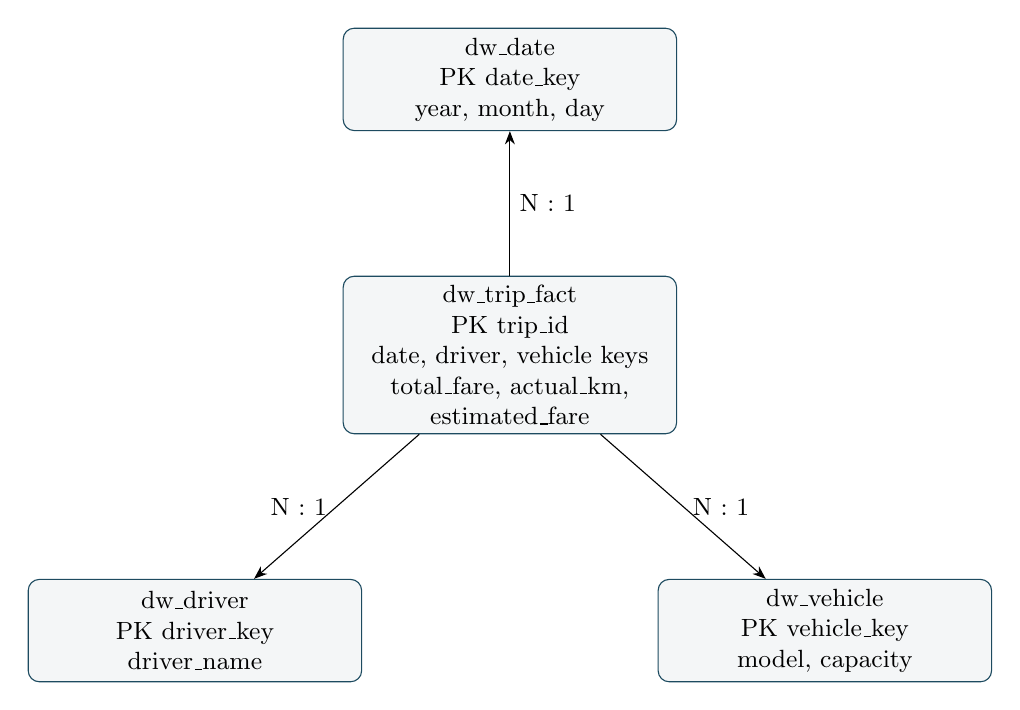
\begin{tikzpicture}[>=Stealth,box/.style={draw=accent,fill=accent!5,rounded corners,align=center,text width=4cm,minimum height=1.3cm,font=\small}]
\node[box](f)at(0,0){dw\_trip\_fact\\PK trip\_id\\date, driver, vehicle keys\\total\_fare, actual\_km, estimated\_fare};
\node[box](d)at(0,3.5){dw\_date\\PK date\_key\\year, month, day};
\node[box](r)at(-4,-3.5){dw\_driver\\PK driver\_key\\driver\_name};
\node[box](v)at(4,-3.5){dw\_vehicle\\PK vehicle\_key\\model, capacity};
\draw[->](f)--node[right,font=\small]{N : 1}(d);\draw[->](f)--node[left,font=\small]{N : 1}(r);\draw[->](f)--node[right,font=\small]{N : 1}(v);
\end{tikzpicture}\end{center}
The executed ROLLUP query groups by completion year, month and vehicle model. It yields model details, monthly subtotals, annual subtotals and a grand total. In this one-month dataset the last three totals happen to match. NULL in those output grouping columns denotes a subtotal level, not a missing dimension value. The dimension source columns are non-null.

The analytical fact has 130 rows, equal to CompletedTrip. Its total fare is 7853.92, exactly matching trip\_\allowbreak{}financials. Each trip identifier is unique, and optional surcharge and review joins are checked not to multiply fact rows. These reconciliations guard against a common analytical error: an apparently plausible sum inflated by a one-to-many join.

Additional delivered queries use LAG to compare adjacent observed completion days and a scalar subquery with HAVING to select drivers whose mean fare exceeds the overall completed-trip mean. LAG means the previous observed date; if a day is absent, it is not automatically the previous calendar day. The complete query output is saved in TSV and JSON files.

\begin{lstlisting}
SELECT d.calendar_year,d.calendar_month,v.model,
 COUNT(*) AS trips,SUM(f.total_fare) AS gross_fare
FROM dw_trip_fact f
JOIN dw_date d ON d.date_key=f.date_key
JOIN dw_vehicle v ON v.vehicle_key=f.vehicle_key
GROUP BY d.calendar_year,d.calendar_month,v.model WITH ROLLUP;
\end{lstlisting}
\par\begingroup\small\noindent
\begin{tabularx}{\linewidth}{YYYYY}
\toprule
Year & Month & Model & Trips & Fare\\\midrule
2026 & 10 & Electric & 39 & 2053.68\\
2026 & 10 & MPV & 45 & 2722.32\\
2026 & 10 & Sedan & 46 & 3077.92\\
2026 & 10 & NULL & 130 & 7853.92\\
2026 & NULL & NULL & 130 & 7853.92\\
NULL & NULL & NULL & 130 & 7853.92\\
\bottomrule
\end{tabularx}
\par\endgroup

\subsection{Design limitations and conclusion}
The strongest improvement over the starting design is consistency across requirements, diagrams, relational keys and executable behavior. A booking can now exist before assignment, each served trip identifies a vehicle, terminal outcomes are distinguished from all unfinished trips, and normalization claims are tied to explicit dependencies.

The fixed vehicle-owner rule is a deliberate simplification that supports a small, coherent schema. It should not be generalized to a platform where vehicles are shared among drivers over time. A temporal assignment model would be the first structural extension in that setting. Similarly, one bilateral review row is convenient for one passenger and one driver per trip; repeated reviews, moderation and revision history would require additional structure.

The application role protects workflow integrity, but it is a service-level role, not per-customer authorization. An application must still verify that an authenticated person is allowed to review a particular trip or read personal information. Authentication, row-level access, encryption policy, retention and production monitoring are outside this database demonstration.

Shift overlaps, driver availability across trips, active insurance at dispatch and customer cancellation fees are not automatically enforced. The stored records make some related queries possible, but data storage should not be mistaken for a completed policy engine. Financial records also do not prove money was paid or settled.

The dataset is small, generated and deliberately covers edge cases. Execution plans are informative about chosen access paths, not benchmarks. The tested concurrency case is limited to two simultaneous completions of one trip. A deployable system would need load testing, failure recovery, operational access controls, richer state transitions and representative data.

Within these limits, the project completes the required path from business requirements through conceptual and logical design to executable implementation and data-use discussion. The analytical extension illustrates the different goals of OLTP and OLAP without replacing the operational model.


\appendix
\clearpage
\section{Data Dictionary}
The definitions below are extracted from the running database's information\_\allowbreak{}schema, so they describe the executed schema rather than an independently maintained design. PRI denotes a primary-key component; UNI denotes a unique index; MUL denotes an indexed non-unique column and is not itself proof of a foreign key. Foreign-key targets are listed in the mapping section.

All identifiers are supplied explicitly by the data loader; no vendor-specific automatic identity generator is needed. Empty optional values use SQL NULL. Phone numbers are text, and monetary values use DECIMAL to avoid floating-point rounding in financial aggregation.

\begingroup\renewcommand{\arraystretch}{1.08}\titlespacing*{\subsection}{0pt}{7pt}{3pt}\subsection*{app\_\allowbreak{}user}
\par\begingroup\small\noindent
\begin{tabularx}{\linewidth}{p{4.4cm}p{4.0cm}p{1.5cm}X}
\toprule
Column & SQL type & Null & Key\\\midrule
user\_\allowbreak{}id & int & NO & PRI\\
full\_\allowbreak{}name & varchar(80) & NO & —\\
phone & varchar(20) & NO & UNI\\
email & varchar(120) & YES & —\\
birth\_\allowbreak{}date & date & YES & —\\
\bottomrule
\end{tabularx}
\par\endgroup
\subsection*{passenger}
\par\begingroup\small\noindent
\begin{tabularx}{\linewidth}{p{4.4cm}p{4.0cm}p{1.5cm}X}
\toprule
Column & SQL type & Null & Key\\\midrule
passenger\_\allowbreak{}id & int & NO & PRI\\
tier & varchar(10) & NO & —\\
\bottomrule
\end{tabularx}
\par\endgroup
\subsection*{driver}
\par\begingroup\small\noindent
\begin{tabularx}{\linewidth}{p{4.4cm}p{4.0cm}p{1.5cm}X}
\toprule
Column & SQL type & Null & Key\\\midrule
driver\_\allowbreak{}id & int & NO & PRI\\
license\_\allowbreak{}no & varchar(30) & NO & UNI\\
lifetime\_\allowbreak{}km & decimal(12,2) & NO & —\\
\bottomrule
\end{tabularx}
\par\endgroup
\endgroup
\begingroup\renewcommand{\arraystretch}{1.08}\titlespacing*{\subsection}{0pt}{7pt}{3pt}\subsection*{vehicle}
\par\begingroup\small\noindent
\begin{tabularx}{\linewidth}{p{4.4cm}p{4.0cm}p{1.5cm}X}
\toprule
Column & SQL type & Null & Key\\\midrule
plate & varchar(12) & NO & PRI\\
driver\_\allowbreak{}id & int & NO & MUL\\
model & varchar(40) & NO & —\\
color & varchar(20) & NO & —\\
capacity & smallint & NO & —\\
\bottomrule
\end{tabularx}
\par\endgroup
\subsection*{insurance\_\allowbreak{}policy}
\par\begingroup\small\noindent
\begin{tabularx}{\linewidth}{p{4.4cm}p{4.0cm}p{1.5cm}X}
\toprule
Column & SQL type & Null & Key\\\midrule
policy\_\allowbreak{}id & int & NO & PRI\\
plate & varchar(12) & NO & MUL\\
valid\_\allowbreak{}from & date & NO & —\\
valid\_\allowbreak{}to & date & NO & —\\
\bottomrule
\end{tabularx}
\par\endgroup
\subsection*{driver\_\allowbreak{}shift}
\par\begingroup\small\noindent
\begin{tabularx}{\linewidth}{p{4.4cm}p{4.0cm}p{1.5cm}X}
\toprule
Column & SQL type & Null & Key\\\midrule
driver\_\allowbreak{}id & int & NO & PRI\\
shift\_\allowbreak{}start & datetime & NO & PRI\\
shift\_\allowbreak{}end & datetime & YES & —\\
\bottomrule
\end{tabularx}
\par\endgroup
\endgroup
\begingroup\renewcommand{\arraystretch}{1.08}\titlespacing*{\subsection}{0pt}{7pt}{3pt}\subsection*{trip}
\par\begingroup\small\noindent
\begin{tabularx}{\linewidth}{p{4.4cm}p{4.0cm}p{1.5cm}X}
\toprule
Column & SQL type & Null & Key\\\midrule
trip\_\allowbreak{}id & int & NO & PRI\\
passenger\_\allowbreak{}id & int & NO & MUL\\
plate & varchar(12) & YES & MUL\\
requested\_\allowbreak{}at & datetime & NO & —\\
started\_\allowbreak{}at & datetime & YES & —\\
origin\_\allowbreak{}zone & varchar(30) & NO & —\\
destination\_\allowbreak{}zone & varchar(30) & NO & —\\
service\_\allowbreak{}type & varchar(12) & NO & —\\
estimated\_\allowbreak{}km & decimal(8,2) & NO & —\\
estimated\_\allowbreak{}fare & decimal(10,2) & NO & —\\
status & varchar(12) & NO & MUL\\
\bottomrule
\end{tabularx}
\par\endgroup
\endgroup
\begingroup\renewcommand{\arraystretch}{1.08}\titlespacing*{\subsection}{0pt}{7pt}{3pt}\subsection*{completed\_\allowbreak{}trip}
\par\begingroup\small\noindent
\begin{tabularx}{\linewidth}{p{4.4cm}p{4.0cm}p{1.5cm}X}
\toprule
Column & SQL type & Null & Key\\\midrule
trip\_\allowbreak{}id & int & NO & PRI\\
ended\_\allowbreak{}at & datetime & NO & —\\
base\_\allowbreak{}fare & decimal(10,2) & NO & —\\
tip & decimal(10,2) & NO & —\\
actual\_\allowbreak{}km & decimal(8,2) & NO & —\\
\bottomrule
\end{tabularx}
\par\endgroup
\subsection*{cancelled\_\allowbreak{}trip}
\par\begingroup\small\noindent
\begin{tabularx}{\linewidth}{p{4.4cm}p{4.0cm}p{1.5cm}X}
\toprule
Column & SQL type & Null & Key\\\midrule
trip\_\allowbreak{}id & int & NO & PRI\\
cancelled\_\allowbreak{}at & datetime & NO & —\\
reason & varchar(160) & NO & —\\
\bottomrule
\end{tabularx}
\par\endgroup
\subsection*{review}
\par\begingroup\small\noindent
\begin{tabularx}{\linewidth}{p{4.4cm}p{4.0cm}p{1.5cm}X}
\toprule
Column & SQL type & Null & Key\\\midrule
trip\_\allowbreak{}id & int & NO & PRI\\
passenger\_\allowbreak{}score & smallint & YES & —\\
passenger\_\allowbreak{}comment & varchar(200) & YES & —\\
driver\_\allowbreak{}score & smallint & YES & —\\
driver\_\allowbreak{}comment & varchar(200) & YES & —\\
\bottomrule
\end{tabularx}
\par\endgroup
\subsection*{surcharge}
\par\begingroup\small\noindent
\begin{tabularx}{\linewidth}{p{4.4cm}p{4.0cm}p{1.5cm}X}
\toprule
Column & SQL type & Null & Key\\\midrule
trip\_\allowbreak{}id & int & NO & PRI\\
amount & decimal(10,2) & NO & —\\
\bottomrule
\end{tabularx}
\par\endgroup
\endgroup
\clearpage
\section{References and Reproduction}
The project requirement asks for context and requirements, ER/EER design, relational design, implementation, and discussion of database construction and data usage. The report's sections follow that sequence. The following mapping identifies how the available lectures inform the work. Lecture 1 was not present among the supplied files; no specific requirement is attributed to an unseen lecture.

The original ride-hailing document is the starting design. Terminology referring to an online shopping mall has been removed. No additional mandatory entity count, UI implementation, or warehouse delivery requirement is inferred from classroom examples; the warehouse is a bounded analytical extension.

\par\begingroup\small\noindent
\begin{tabularx}{\linewidth}{YY}
\toprule
Source & Applied concepts\\\midrule
Group Project Requirements, Fall 2026 & Five development components and depth/reliability criteria\\
LN2 Relational data model & Domains, keys, integrity and business context\\
LN3 Conceptual model and ER diagrams I & Entities, attributes, cardinality, weak entities\\
LN4 Conceptual model and ER diagrams II & Partial/total and overlapping/disjoint specialization\\
LN5 Logical design and theory I & Entity/relationship/subtype mapping to relations\\
LN6 Logical design and theory II & Functional dependencies, 1NF, 2NF, 3NF and BCNF\\
LN7 SQL basic & MySQL DDL, constraints and CRUD\\
LN8 SQL basic & NULL, joins, aggregation, filtering and subqueries\\
LN9 Advanced SQL & Views, advanced queries and transactions\\
LN10 Data Warehouse & OLTP/OLAP, star schema, ROLLUP and LAG\\
\bottomrule
\end{tabularx}
\par\endgroup
\subsection*{Implementation references}
\begin{itemize}\small
\item MySQL 8.4 Reference Manual, \emph{CHECK Constraints}: \url{https://dev.mysql.com/doc/refman/8.4/en/create-table-check-constraints.html}.
\item MySQL 8.4 Reference Manual, \emph{Locking Reads}: \url{https://dev.mysql.com/doc/refman/8.4/en/innodb-locking-reads.html}.
\item MySQL 8.4 Reference Manual, \emph{GROUP BY Modifiers}: \url{https://dev.mysql.com/doc/refman/8.4/en/group-by-modifiers.html}.
\end{itemize}
Use a disposable MySQL 8.4 instance with an empty schema namespace. The schema script intentionally fails if ride\_\allowbreak{}hailing already exists; it does not silently erase an existing database. Run the schema, routines, generated seed, warehouse and role scripts in order, then run the validation program. The README supplies commands and explains the dedicated instance setup.

The SQL scripts are the executable source of truth. create\_\allowbreak{}logic.py regenerates procedure definitions, generate\_\allowbreak{}data.py regenerates the same sample data, and run\_\allowbreak{}validation.py reruns checks and collects query outputs. build\_\allowbreak{}reports.py reads those outputs and the actual information\_\allowbreak{}schema export to create both LaTeX versions. The supplied .tex files can also be compiled directly with XeLaTeX.

The successful verification used MySQL 8.4.13 in an isolated temporary directory with TCP networking disabled. The local sandbox could not initialize or access the server normally; the database was therefore run outside that restriction with access limited to its local socket. This is an environment detail, not an unexecuted-test exception. All published checks actually ran.

The report includes selected SQL and result tables for readability. Full scripts, raw query outputs, test records and a server-derived data dictionary are supplied so that design claims can be checked independently.

\par\begingroup\small\noindent
\begin{tabularx}{\linewidth}{YY}
\toprule
File or directory & Purpose\\\midrule
report\_\allowbreak{}en.pdf / report\_\allowbreak{}zh.pdf & English report and Chinese counterpart\\
source/report\_\allowbreak{}en.tex / report\_\allowbreak{}zh.tex & Editable LaTeX sources\\
sql/01\_\allowbreak{}schema.sql … 07\_\allowbreak{}report\_\allowbreak{}demonstrations.sql & Operational schema, lifecycle, data, warehouse, queries, role\\
scripts/ & Generation, validation, report build and execution helpers\\
results/validation.json & 32 pass/fail records and error evidence\\
results/query\_\allowbreak{}results.json and *.tsv & Actual query outputs, including EXPLAIN\\
results/report\_\allowbreak{}evidence.json & Table samples and CRUD results\\
figures/ & Four diagrams: PDF, SVG, PNG and editable draw.io\\
results/data\_\allowbreak{}dictionary.tsv & Executed column metadata\\
README.md & Reproduction instructions and compatibility notes\\
\bottomrule
\end{tabularx}
\par\endgroup

\clearpage
\section{Team Responsibilities (Draft)}
This working table records the scope confirmed so far. It is not a peer-assessment score sheet and does not replace the separate Group Project Contribution Form referenced by the project requirements. Duties for the other five members remain unassigned in this draft; no contribution percentages are inferred.

Lin Shuaiyu confirmed responsibility for defining the overall report topic, requirements and business scope, conceptual ER/EER design, and logical design including relational mapping and normalization, up to the stage before concrete sample-data preparation. Possible later work on data generation, implementation or integration is not listed as a confirmed responsibility here.

\par\begingroup\small\noindent
\begin{tabularx}{\linewidth}{p{2.7cm}p{3cm}X}
\toprule
Member & Student ID & Confirmed scope / placeholder\\\midrule
Lin Shuaiyu & 226040384 & Topic definition; requirements and scope; ER/EER design; relational mapping and normalization.\\
Cai Ruihe & 226040421 & TBD - placeholder; not yet assigned.\\
Li Songzi & 226040351 & TBD - placeholder; not yet assigned.\\
Wen Zhang & 226040373 & TBD - placeholder; not yet assigned.\\
Zhang Xiujie & 226040424 & TBD - placeholder; not yet assigned.\\
Jin Conghao & 122090871 & TBD - placeholder; not yet assigned.\\
\bottomrule
\end{tabularx}
\par\endgroup
\end{document}
